\paragraph{} Neste capítulo serão apresentados os resultados do modelo, avaliado pelas medidas de desempenho descritas anteriormente, junto com os gráficos da previsão do conjunto de teste.

\paragraph{} Os resultados serão apresentados para cada modelo, com os dois conjuntos de dados disponíveis: Biodiesel Nacional e Óleo de Soja e as duas abordagens de pré-processamento: remoção de tendência linear e normalização min-max. Os diferentes tipos de janelamento: Janela deslizante e Janela de Takens serão considerados modelos distintos.

\section{Janela Deslizante}

\paragraph{} Os resultados obtidos pelo modelo utilizando a abordagem de janela deslizante são apresentados nas Tabelas \ref{tab:resultados_validacao} e \ref{tab:resultados_teste}, que detalham as métricas de desempenho para cada cenário avaliado, tanto na validação cruzada quanto no conjunto de teste. Além disso, as Figuras \ref{fig:brasil_results}, \ref{fig:brasil_oil_results}, \ref{fig:brasil_results_test} e \ref{fig:brasil_oil_results_test} ilustram essa comparação de forma gráfica, representando os mesmos dados das tabelas em gráficos de pontos.
\paragraph{} As subseções a seguir discutem os resultados de cada modelo, abordando os gráficos de previsão e a distribuição dos resíduos. Serão apresentadas as previsões comparadas aos valores reais, além da análise da distribuição dos resíduos por meio de histogramas e gráficos de dispersão, com o objetivo de compreender o comportamento do modelo e avaliar sua adequação aos dados.

\subsection{\acs{NARX}}
\paragraph{} Conforme apresentado na Figura \ref{fig:narx_results} destaca-se que o modelo (b) foi o único capaz de mapear os dados reais de forma satisfatória, apresentando baixos valores de erro no conjunto de teste e mantendo essa performance de forma consistente no conjunto de desenvolvimento. Os resultados obtidos indicam que o desvio padrão dos erros foi inferior a 10\% das respectivas medidas, como detalhado nas Tabelas \ref{tab:resultados_validacao} e \ref{tab:resultados_teste}. Apesar do desempenho insatisfatório dos modelos (c) e (d), observa-se que ambos mantiveram consistência ao longo das validações.
\paragraph{} Além disso, ao analisar os gráficos de dispersão apresentados na Figura \ref{fig:narx_scatter}, observou-se que o modelo (b) exibe uma dispersão reduzida, evidenciando uma correlação positiva clara entre os valores previstos e observados. Em contraste, os modelos (a) e (c) demonstram maior dispersão para valores menores e uma redução dessa dispersão à medida que os valores aumentam, com uma linha de tendência também positiva. O modelo (d), por sua vez, apresenta uma dispersão considerável ao longo de todo o intervalo de valores, sem uma clara tendência.
\paragraph{} Por fim, os histogramas dos resíduos, ilustrados na Figura \ref{fig:narx_residuals_histogram}, revelam que o modelo (b) gera uma distribuição dos resíduos mais próxima de uma distribuição normal, embora com alguns valores discrepantes próximos a 0,2 e 0,3, que deslocam a média para a direita. Em contrapartida, os modelos (a), (c) e (d) exibem distribuições assimétricas, com a presença de valores discrepantes mais pronunciados, indicando um comportamento menos ideal na previsão dos resíduos.

\begin{figure}[htbp]
	\centering
	\begin{subfigure}[b]{0.45\textwidth}
		\centering
		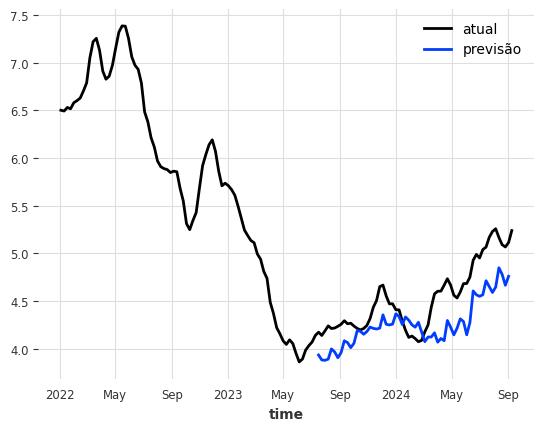
\includegraphics[width=\textwidth]{figuras/narx_brasil_plot.png} % Substitua pelo caminho da sua imagem
		\caption{Treinado com Biodiesel Nacional \newline}
		\label{fig:narx_brasil_plot}
	\end{subfigure}
	\hfill
	\begin{subfigure}[b]{0.45\textwidth}
		\centering
		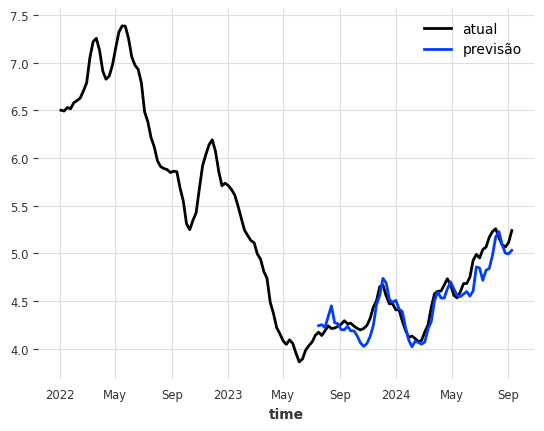
\includegraphics[width=\textwidth]{figuras/narx_brasil_oil_plot.png} % Substitua pelo caminho da sua imagem
		\caption{Treinado com Biodiesel Nacional e Óleo de Soja}
		\label{fig:narx_brasil_oil_plot}
	\end{subfigure}

	\vskip\baselineskip % Espaçamento vertical entre as linhas de imagens

	\begin{subfigure}[b]{0.45\textwidth}
		\centering
		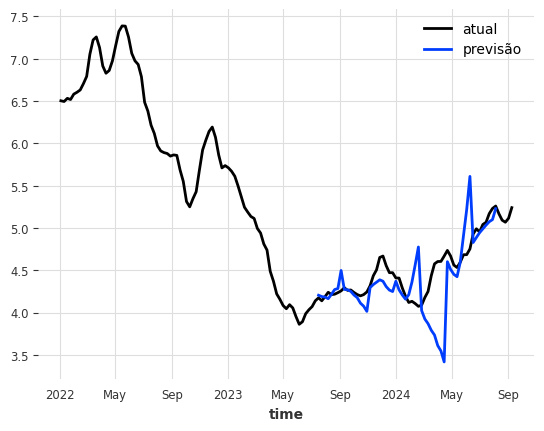
\includegraphics[width=\textwidth]{figuras/narx_brasil_detrend_plot.png} % Substitua pelo caminho da sua imagem
		\caption{Treinado com Biodiesel Nacional sem tendência}
		\label{fig:narx_brasil_detrend_plot}
	\end{subfigure}
	\hfill
	\begin{subfigure}[b]{0.45\textwidth}
		\centering
		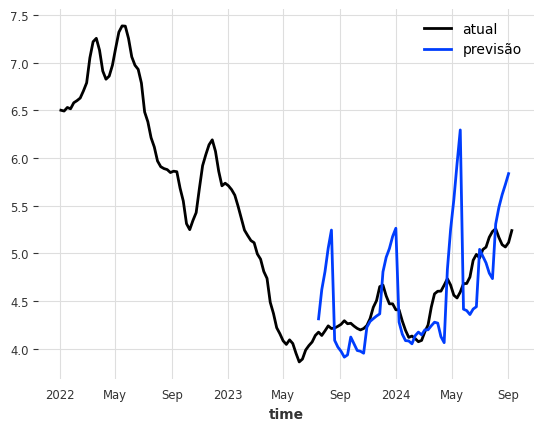
\includegraphics[width=\textwidth]{figuras/narx_brasil_oil_detrend_plot.png} % Substitua pelo caminho da sua imagem
		\caption{Treinado com Biodiesel Nacional e Óleo de Soja sem tendência}
		\label{fig:narx_brasil_oil_detrend_plot}
	\end{subfigure}

	\caption{Resultados do modelo \acs{NARX} no conjunto de teste}
	\label{fig:narx_results}
\end{figure}
\begin{figure}[htbp]
	\centering
	\begin{subfigure}[b]{0.40\textwidth}
		\centering
		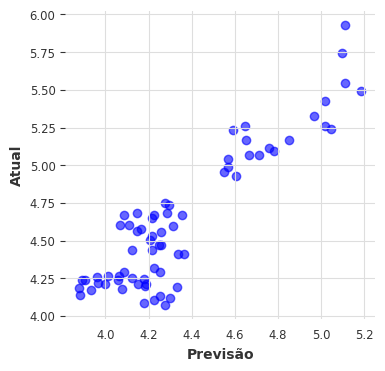
\includegraphics[width=\textwidth]{figuras/narx_brasil_scatter.png} % Substitua pelo caminho da sua imagem
		\caption{Treinado com Biodiesel Nacional \newline}
		\label{fig:narx_brasil_scatter}
	\end{subfigure}
	\hfill
	\begin{subfigure}[b]{0.40\textwidth}
		\centering
		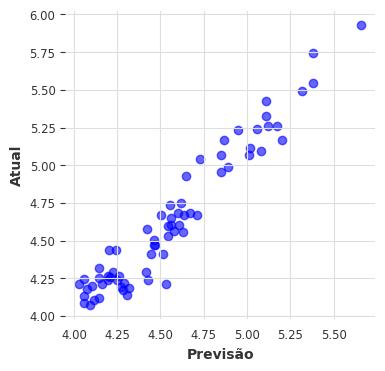
\includegraphics[width=\textwidth]{figuras/narx_brasil_oil_scatter.png} % Substitua pelo caminho da sua imagem
		\caption{Treinado com Biodiesel Nacional e Óleo de Soja}
		\label{fig:narx_brasil_oil_scatter}
	\end{subfigure}

	\vskip\baselineskip % Espaçamento vertical entre as linhas de imagens

	\begin{subfigure}[b]{0.40\textwidth}
		\centering
		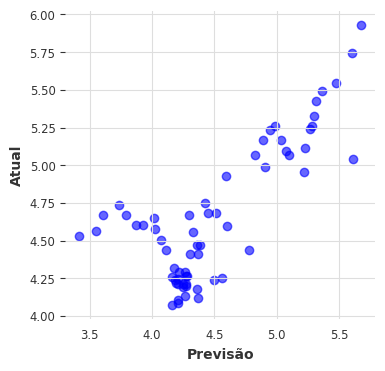
\includegraphics[width=\textwidth]{figuras/narx_brasil_detrend_scatter.png} % Substitua pelo caminho da sua imagem
		\caption{Treinado com Biodiesel Nacional sem tendência}
		\label{fig:narx_brasil_detrend_scatter}
	\end{subfigure}
	\hfill
	\begin{subfigure}[b]{0.40\textwidth}
		\centering
		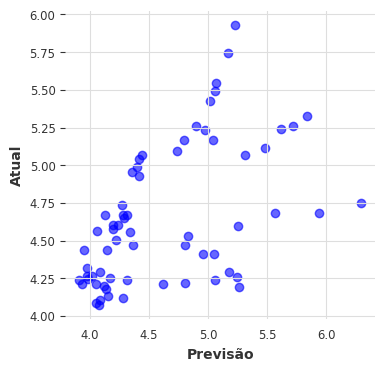
\includegraphics[width=\textwidth]{figuras/narx_brasil_oil_detrend_scatter.png} % Substitua pelo caminho da sua imagem
		\caption{Treinado com Biodiesel Nacional e Óleo de Soja sem tendência}
		\label{fig:narx_brasil_oil_detrend_scatter}
	\end{subfigure}

	\caption{Gráficos de dispersão dos valores atuais versus valores previstos pelo modelo \acs{NARX} no conjunto de teste}
	\label{fig:narx_scatter}
\end{figure}
\begin{figure}[htbp]
	\centering
	\begin{subfigure}[b]{0.40\textwidth}
		\centering
		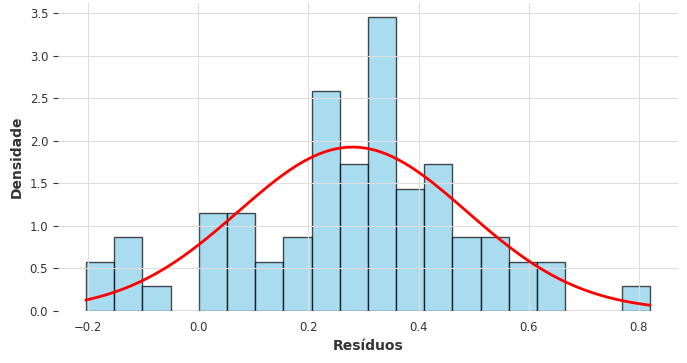
\includegraphics[width=\textwidth]{figuras/narx_brasil_residuals_histogram.png} % Substitua pelo caminho da sua imagem
		\caption{Treinado com Biodiesel Nacional \newline}
		\label{fig:narx_brasil_residuals_histogram}
	\end{subfigure}
	\hfill
	\begin{subfigure}[b]{0.40\textwidth}
		\centering
		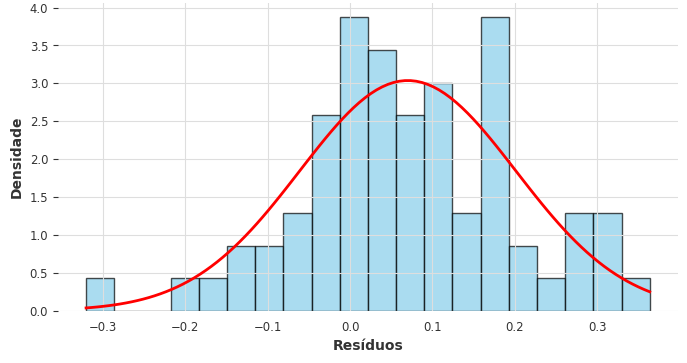
\includegraphics[width=\textwidth]{figuras/narx_brasil_oil_residuals_histogram.png} % Substitua pelo caminho da sua imagem
		\caption{Treinado com Biodiesel Nacional e Óleo de Soja}
		\label{fig:narx_brasil_oil_residuals_histogram}
	\end{subfigure}

	\vskip\baselineskip % Espaçamento vertical entre as linhas de imagens

	\begin{subfigure}[b]{0.40\textwidth}
		\centering
		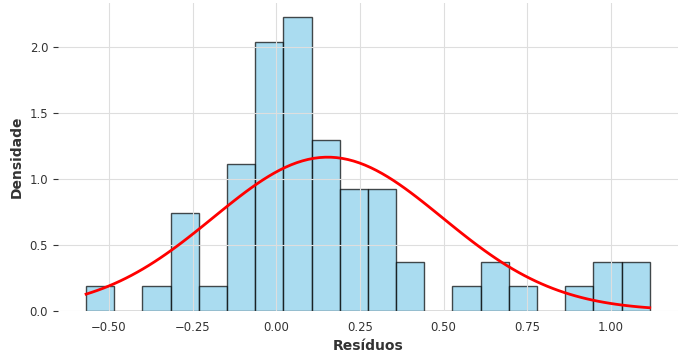
\includegraphics[width=\textwidth]{figuras/narx_brasil_detrend_residuals_histogram.png} % Substitua pelo caminho da sua imagem
		\caption{Treinado com Biodiesel Nacional sem tendência}
		\label{fig:narx_brasil_detrend_residuals_histogram}
	\end{subfigure}
	\hfill
	\begin{subfigure}[b]{0.40\textwidth}
		\centering
		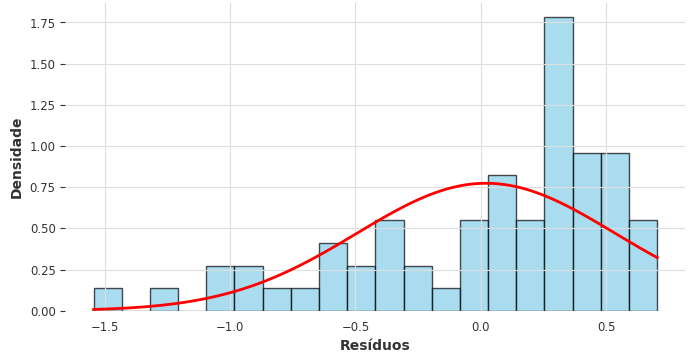
\includegraphics[width=\textwidth]{figuras/narx_brasil_oil_detrend_residuals_histogram.png} % Substitua pelo caminho da sua imagem
		\caption{Treinado com Biodiesel Nacional e Óleo de Soja sem tendência}
		\label{fig:narx_brasil_oil_detrend_residuals_histogram}
	\end{subfigure}

	\caption{Histograma dos erros do modelo \acs{NARX} no conjunto de teste}
	\label{fig:narx_residuals_histogram}
\end{figure}

\subsection{\acs{DA-RNN}}
\paragraph{} Como ilustrado na Figura \ref{fig:darnn_results}, o modelo (c) apresentou uma capacidade eficaz de mapeamento, reproduzindo de forma precisa os dados reais e alcançando baixos valores de erro no conjunto de teste, conforme exposto na Tabela \ref{tab:resultados_teste}. Contudo, os resultados obtidos no conjunto de desenvolvimento revelaram-se inconsistentes, sugerindo um possível superdimensionamento do modelo para este conjunto de dados, conforme indicado pela Tabela \ref{tab:resultados_validacao}. Ao comparar os resultados das Tabelas \ref{tab:resultados_validacao} e \ref{tab:resultados_teste}, nota-se uma inversão no desempenho: enquanto o modelo (c) obteve o melhor resultado no conjunto de teste, apresentou o pior desempenho no conjunto de desenvolvimento, ao passo que o modelo (d) demonstrou o comportamento oposto, que novamente sugere um superdimensionamento do modelo.
\paragraph{} Adicionalmente, ao examinar os gráficos de dispersão apresentados na Figura \ref{fig:darnn_scatter}, observou-se que o modelo (c) apresenta uma dispersão reduzida, o que indica uma correlação positiva clara entre os valores previstos e observados. Em contraste, os modelos (a), (b) e (d) exibem uma maior dispersão para valores mais baixos, com uma diminuição dessa dispersão à medida que os valores aumentam, sendo que a linha de tendência, embora também positiva, possui uma inclinação ligeiramente inferior a 1, sugerindo um aumento do erro conforme os valores reais se elevam.
\paragraph{} Por último, conforme ilustrado na Figura \ref{fig:darnn_residuals_histogram}, os histogramas dos resíduos indicam que o modelo (c) gera uma distribuição dos resíduos que se aproxima de uma distribuição normal, com um leve desvio para a direita. Em contrapartida, os modelos (a), (b) e (d) apresentam distribuições com caudas pesadas, sugerindo maior variabilidade nos erros de previsão.
\begin{figure}[htbp]
	\centering
	\begin{subfigure}[b]{0.45\textwidth}
		\centering
		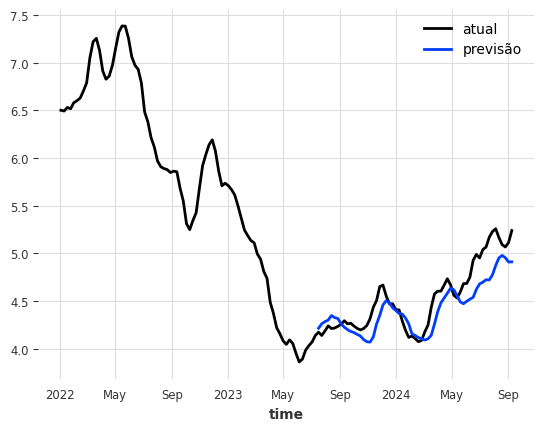
\includegraphics[width=\textwidth]{figuras/darnn_brasil_plot.png} % Substitua pelo caminho da sua imagem
		\caption{Treinado com Biodiesel Nacional \newline}
		\label{fig:darnn_brasil_plot}
	\end{subfigure}
	\hfill
	\begin{subfigure}[b]{0.45\textwidth}
		\centering
		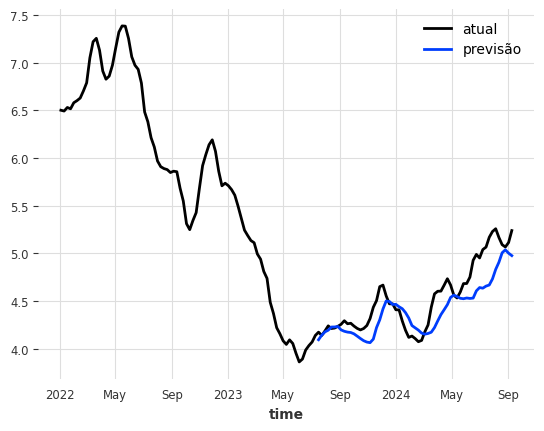
\includegraphics[width=\textwidth]{figuras/darnn_brasil_oil_plot.png} % Substitua pelo caminho da sua imagem
		\caption{Treinado com Biodiesel Nacional e Óleo de Soja}
		\label{fig:darnn_brasil_oil_plot}
	\end{subfigure}

	\vskip\baselineskip % Espaçamento vertical entre as linhas de imagens

	\begin{subfigure}[b]{0.45\textwidth}
		\centering
		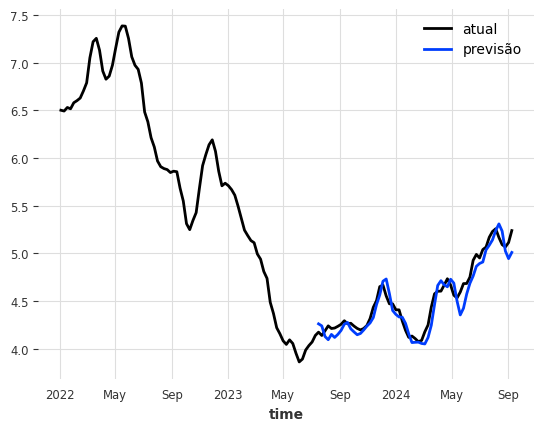
\includegraphics[width=\textwidth]{figuras/darnn_brasil_detrend_plot.png} % Substitua pelo caminho da sua imagem
		\caption{Treinado com Biodiesel Nacional sem tendência}
		\label{fig:darnn_brasil_detrend_plot}
	\end{subfigure}
	\hfill
	\begin{subfigure}[b]{0.45\textwidth}
		\centering
		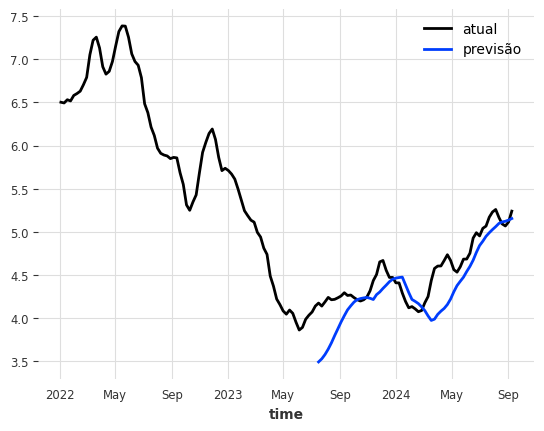
\includegraphics[width=\textwidth]{figuras/darnn_brasil_oil_detrend_plot.png} % Substitua pelo caminho da sua imagem
		\caption{Treinado com Biodiesel Nacional e Óleo de Soja sem tendência}
		\label{fig:darnn_brasil_oil_detrend_plot}
	\end{subfigure}

	\caption{Resultados do modelo \acs{DA-RNN} no conjunto de teste}
	\label{fig:darnn_results}
\end{figure}
\begin{figure}[htbp]
	\centering
	\begin{subfigure}[b]{0.40\textwidth}
		\centering
		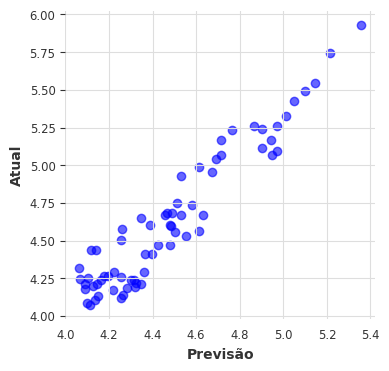
\includegraphics[width=\textwidth]{figuras/darnn_brasil_scatter.png} % Substitua pelo caminho da sua imagem
		\caption{Treinado com Biodiesel Nacional \newline}
		\label{fig:darnn_brasil_scatter}
	\end{subfigure}
	\hfill
	\begin{subfigure}[b]{0.40\textwidth}
		\centering
		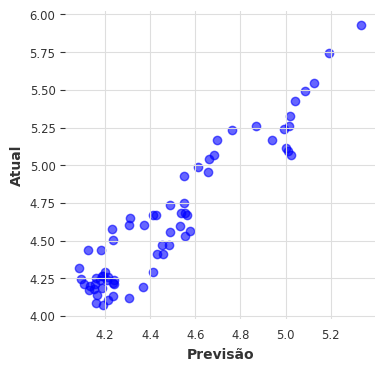
\includegraphics[width=\textwidth]{figuras/darnn_brasil_oil_scatter.png} % Substitua pelo caminho da sua imagem
		\caption{Treinado com Biodiesel Nacional e Óleo de Soja}
		\label{fig:darnn_brasil_oil_scatter}
	\end{subfigure}

	\vskip\baselineskip % Espaçamento vertical entre as linhas de imagens

	\begin{subfigure}[b]{0.40\textwidth}
		\centering
		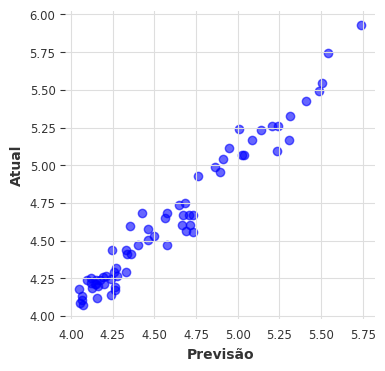
\includegraphics[width=\textwidth]{figuras/darnn_brasil_detrend_scatter.png} % Substitua pelo caminho da sua imagem
		\caption{Treinado com Biodiesel Nacional sem tendência}
		\label{fig:darnn_brasil_detrend_scatter}
	\end{subfigure}
	\hfill
	\begin{subfigure}[b]{0.40\textwidth}
		\centering
		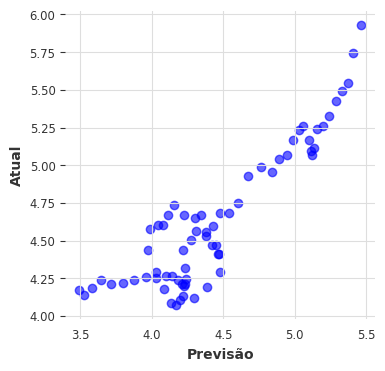
\includegraphics[width=\textwidth]{figuras/darnn_brasil_oil_detrend_scatter.png} % Substitua pelo caminho da sua imagem
		\caption{Treinado com Biodiesel Nacional e Óleo de Soja sem tendência}
		\label{fig:darnn_brasil_oil_detrend_scatter}
	\end{subfigure}

	\caption{Gráficos de dispersão dos valores atuais versus valores previstos pelo modelo \acs{DA-RNN} no conjunto de teste}
	\label{fig:darnn_scatter}
\end{figure}
\begin{figure}[htbp]
	\centering
	\begin{subfigure}[b]{0.40\textwidth}
		\centering
		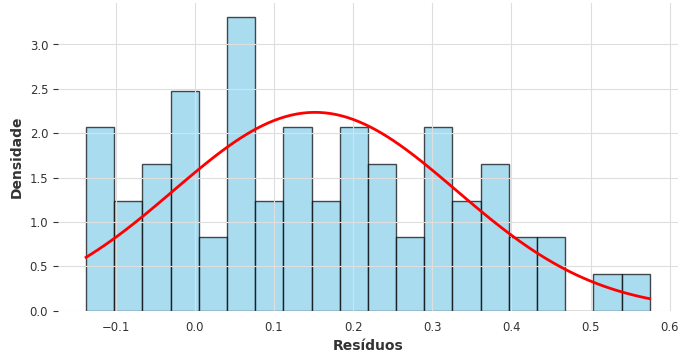
\includegraphics[width=\textwidth]{figuras/darnn_brasil_residuals_histogram.png} % Substitua pelo caminho da sua imagem
		\caption{Treinado com Biodiesel Nacional \newline}
		\label{fig:darnn_brasil_residuals_histogram}
	\end{subfigure}
	\hfill
	\begin{subfigure}[b]{0.40\textwidth}
		\centering
		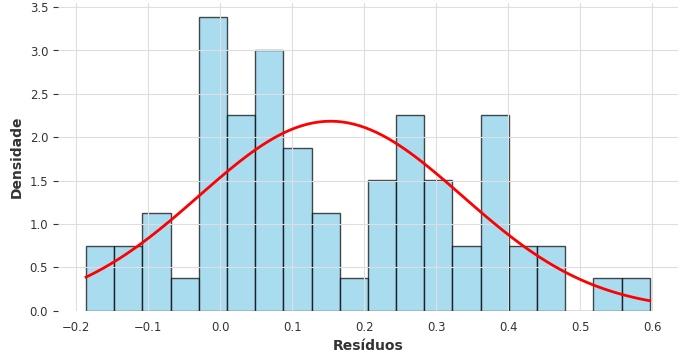
\includegraphics[width=\textwidth]{figuras/darnn_brasil_oil_residuals_histogram.png} % Substitua pelo caminho da sua imagem
		\caption{Treinado com Biodiesel Nacional e Óleo de Soja}
		\label{fig:darnn_brasil_oil_residuals_histogram}
	\end{subfigure}

	\vskip\baselineskip % Espaçamento vertical entre as linhas de imagens

	\begin{subfigure}[b]{0.40\textwidth}
		\centering
		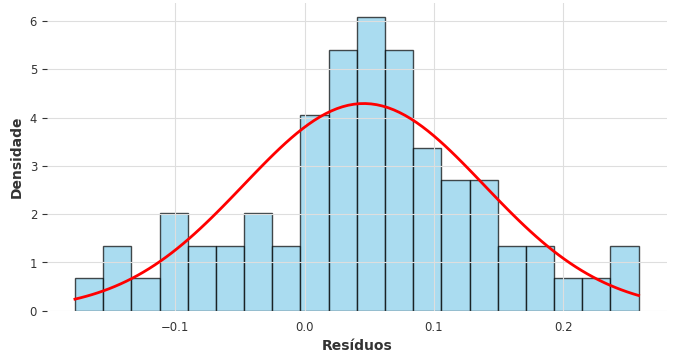
\includegraphics[width=\textwidth]{figuras/darnn_brasil_detrend_residuals_histogram.png} % Substitua pelo caminho da sua imagem
		\caption{Treinado com Biodiesel Nacional sem tendência}
		\label{fig:darnn_brasil_detrend_residuals_histogram}
	\end{subfigure}
	\hfill
	\begin{subfigure}[b]{0.40\textwidth}
		\centering
		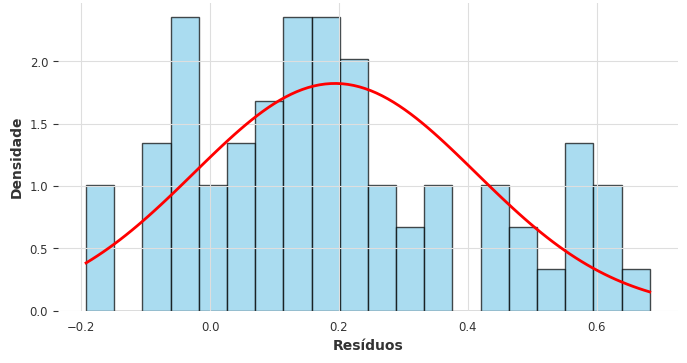
\includegraphics[width=\textwidth]{figuras/darnn_brasil_oil_detrend_residuals_histogram.png} % Substitua pelo caminho da sua imagem
		\caption{Treinado com Biodiesel Nacional e Óleo de Soja sem tendência}
		\label{fig:darnn_brasil_oil_detrend_residuals_histogram}
	\end{subfigure}

	\caption{Histograma dos erros do modelo \acs{DA-RNN} no conjunto de teste}
	\label{fig:darnn_residuals_histogram}
\end{figure}

\subsection{\acs{MLP}}
\paragraph{} Como mostrado na Tabela \ref{tab:resultados_teste} e na Figura \ref{fig:mlp_results}, os modelos (c) e (d) apresentaram os menores valores de erro entre todos os modelos baseados em janela deslizante. No entanto, apenas os modelos (b) e (d), que utilizaram um conjunto de treinamento mais extenso, mostraram resultados consistentes no conjunto de desenvolvimento, como evidenciado na Tabela \ref{tab:resultados_validacao}. Esse desempenho sugere que o tamanho do conjunto de treinamento desempenha um papel importante na capacidade de generalização do modelo.
\paragraph{} Adicionalmente, a análise dos gráficos de dispersão apresentados na Figura \ref{fig:mlp_scatter} revelou que os modelos (c) e (d) exibem uma dispersão reduzida, com correlação próxima de 1, indicando um bom ajuste entre os valores previstos e observados. Em contraste, os modelos (a) e (b) apresentaram maior dispersão, com as linhas de tendência mostrando uma inclinação ligeiramente superior a 1, sugerindo um aumento no erro conforme os valores reais aumentam.
\paragraph{} Por fim, ao examinar os histogramas dos resíduos, apresentados na Figura \ref{fig:mlp_residuals_histogram}, observou-se que os modelos (a), (b) e (d) exibem distribuições que se aproximam de uma distribuição normal, embora com a presença de múltiplos picos. Em contrapartida, o modelo (c) demonstrou uma distribuição assimétrica, com maior concentração de resíduos em torno de zero.

\begin{figure}[htbp]
	\centering
	\begin{subfigure}[b]{0.45\textwidth}
		\centering
		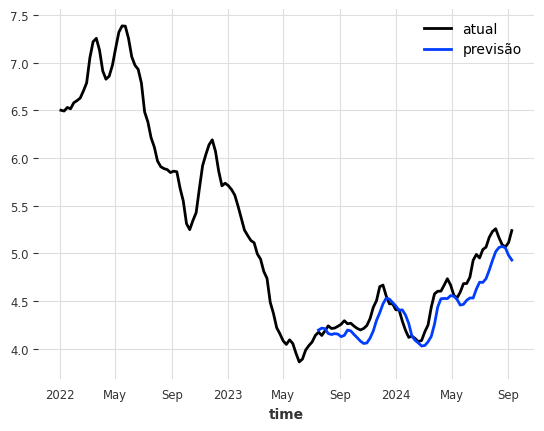
\includegraphics[width=\textwidth]{figuras/mlp_brasil_plot.png} % Substitua pelo caminho da sua imagem
		\caption{Treinado com Biodiesel Nacional \newline}
		\label{fig:mlp_brasil_plot}
	\end{subfigure}
	\hfill
	\begin{subfigure}[b]{0.45\textwidth}
		\centering
		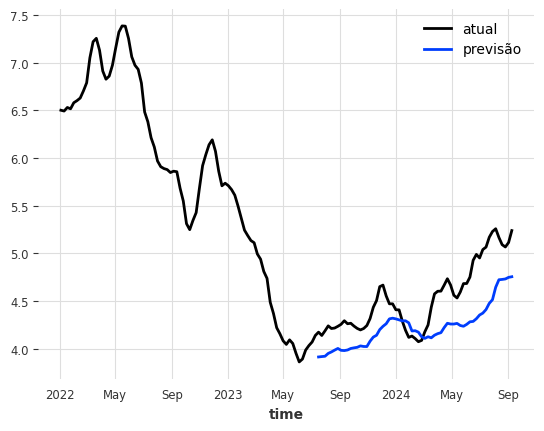
\includegraphics[width=\textwidth]{figuras/mlp_brasil_oil_plot.png} % Substitua pelo caminho da sua imagem
		\caption{Treinado com Biodiesel Nacional e Óleo de Soja}
		\label{fig:mlp_brasil_oil_plot}
	\end{subfigure}

	\vskip\baselineskip % Espaçamento vertical entre as linhas de imagens

	\begin{subfigure}[b]{0.45\textwidth}
		\centering
		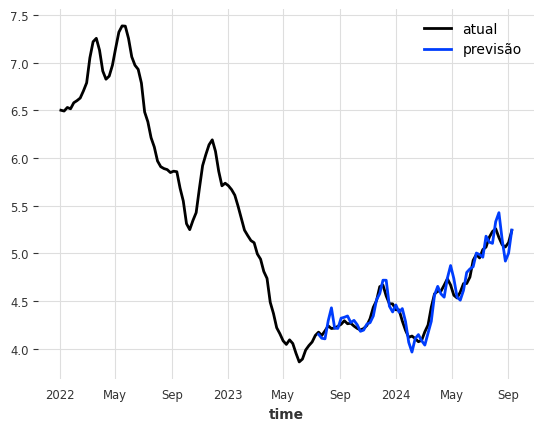
\includegraphics[width=\textwidth]{figuras/mlp_brasil_detrend_plot.png} % Substitua pelo caminho da sua imagem
		\caption{Treinado com Biodiesel Nacional sem tendência}
		\label{fig:mlp_brasil_detrend_plot}
	\end{subfigure}
	\hfill
	\begin{subfigure}[b]{0.45\textwidth}
		\centering
		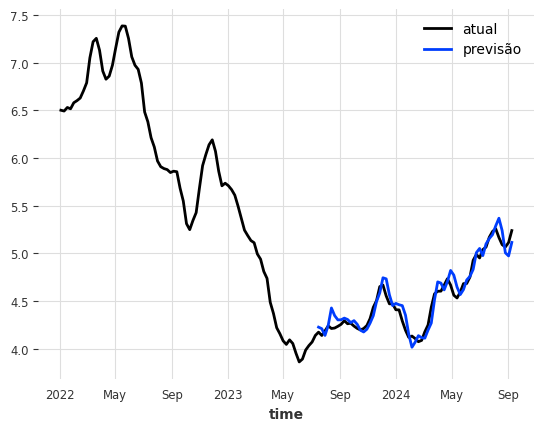
\includegraphics[width=\textwidth]{figuras/mlp_brasil_oil_detrend_plot.png} % Substitua pelo caminho da sua imagem
		\caption{Treinado com Biodiesel Nacional e Óleo de Soja sem tendência}
		\label{fig:mlp_brasil_oil_detrend_plot}
	\end{subfigure}

	\caption{Resultados do modelo \acs{MLP} no conjunto de teste}
	\label{fig:mlp_results}
\end{figure}
\begin{figure}[htbp]
	\centering
	\begin{subfigure}[b]{0.40\textwidth}
		\centering
		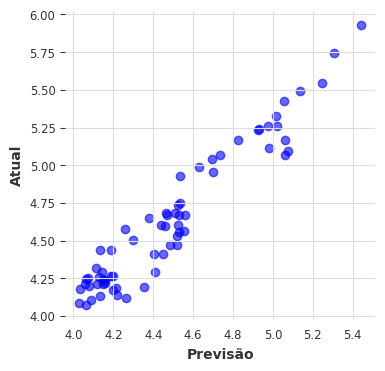
\includegraphics[width=\textwidth]{figuras/mlp_brasil_scatter.png} % Substitua pelo caminho da sua imagem
		\caption{Treinado com Biodiesel Nacional \newline}
		\label{fig:mlp_brasil_scatter}
	\end{subfigure}
	\hfill
	\begin{subfigure}[b]{0.40\textwidth}
		\centering
		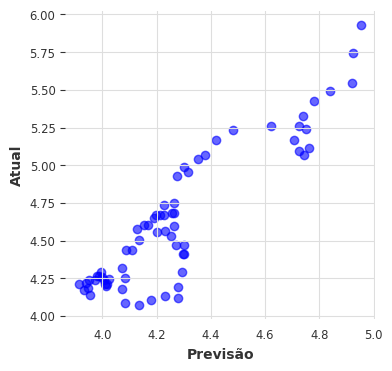
\includegraphics[width=\textwidth]{figuras/mlp_brasil_oil_scatter.png} % Substitua pelo caminho da sua imagem
		\caption{Treinado com Biodiesel Nacional e Óleo de Soja}
		\label{fig:mlp_brasil_oil_scatter}
	\end{subfigure}

	\vskip\baselineskip % Espaçamento vertical entre as linhas de imagens

	\begin{subfigure}[b]{0.40\textwidth}
		\centering
		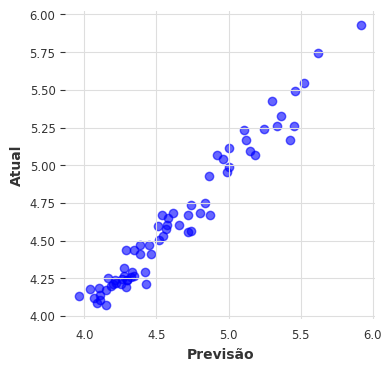
\includegraphics[width=\textwidth]{figuras/mlp_brasil_detrend_scatter.png} % Substitua pelo caminho da sua imagem
		\caption{Treinado com Biodiesel Nacional sem tendência}
		\label{fig:mlp_brasil_detrend_scatter}
	\end{subfigure}
	\hfill
	\begin{subfigure}[b]{0.40\textwidth}
		\centering
		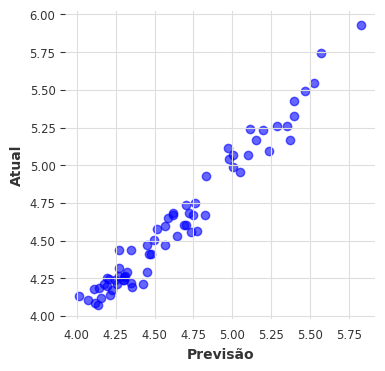
\includegraphics[width=\textwidth]{figuras/mlp_brasil_oil_detrend_scatter.png} % Substitua pelo caminho da sua imagem
		\caption{Treinado com Biodiesel Nacional e Óleo de Soja sem tendência}
		\label{fig:mlp_brasil_oil_detrend_scatter}
	\end{subfigure}

	\caption{Gráficos de dispersão dos valores atuais versus valores previstos pelo modelo \acs{MLP} no conjunto de teste}
	\label{fig:mlp_scatter}
\end{figure}
\begin{figure}[htbp]
	\centering
	\begin{subfigure}[b]{0.40\textwidth}
		\centering
		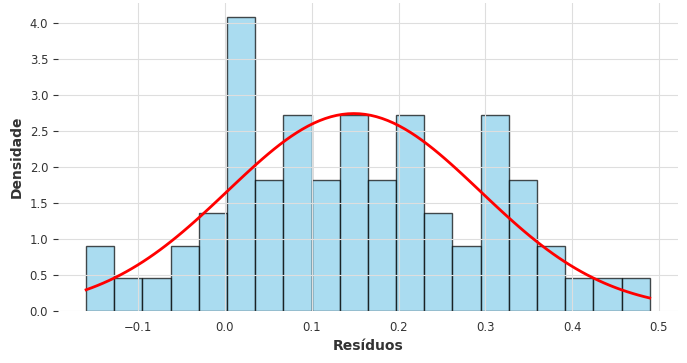
\includegraphics[width=\textwidth]{figuras/mlp_brasil_residuals_histogram.png} % Substitua pelo caminho da sua imagem
		\caption{Treinado com Biodiesel Nacional \newline}
		\label{fig:mlp_brasil_residuals_histogram}
	\end{subfigure}
	\hfill
	\begin{subfigure}[b]{0.40\textwidth}
		\centering
		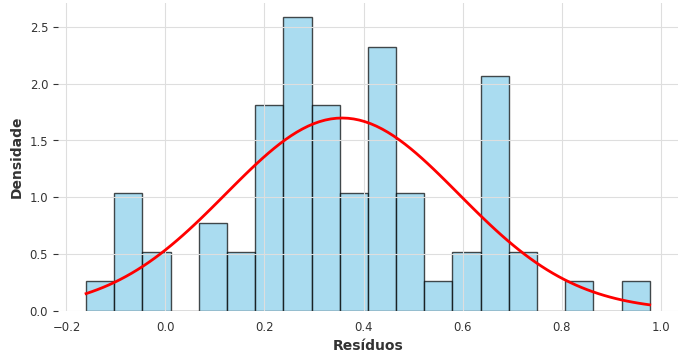
\includegraphics[width=\textwidth]{figuras/mlp_brasil_oil_residuals_histogram.png} % Substitua pelo caminho da sua imagem
		\caption{Treinado com Biodiesel Nacional e Óleo de Soja}
		\label{fig:mlp_brasil_oil_residuals_histogram}
	\end{subfigure}

	\vskip\baselineskip % Espaçamento vertical entre as linhas de imagens

	\begin{subfigure}[b]{0.40\textwidth}
		\centering
		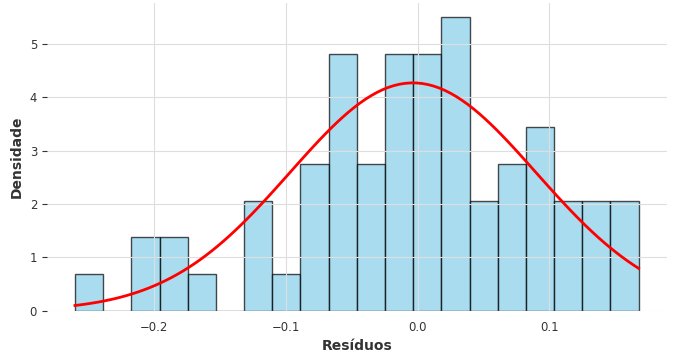
\includegraphics[width=\textwidth]{figuras/mlp_brasil_detrend_residuals_histogram.png} % Substitua pelo caminho da sua imagem
		\caption{Treinado com Biodiesel Nacional sem tendência}
		\label{fig:mlp_brasil_detrend_residuals_histogram}
	\end{subfigure}
	\hfill
	\begin{subfigure}[b]{0.40\textwidth}
		\centering
		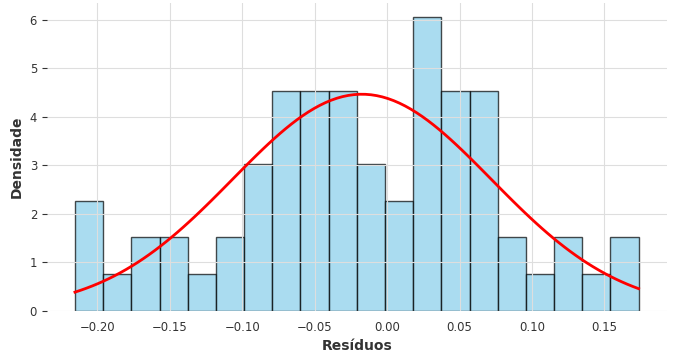
\includegraphics[width=\textwidth]{figuras/mlp_brasil_oil_detrend_residuals_histogram.png} % Substitua pelo caminho da sua imagem
		\caption{Treinado com Biodiesel Nacional e Óleo de Soja sem tendência}
		\label{fig:mlp_brasil_oil_detrend_residuals_histogram}
	\end{subfigure}

	\caption{Histograma dos erros do modelo \acs{MLP} no conjunto de teste}
	\label{fig:mlp_residuals_histogram}
\end{figure}

\subsection{\acs{IMP}}
\paragraph{} O modelo \ac{IMP} apresentou resultados inconsistentes em todos os cenários analisados e não obteve um desempenho satisfatório no conjunto de teste, conforme ilustrado na Figura \ref{fig:imp_results}.
\paragraph{} Adicionalmente, ao examinar os gráficos de dispersão apresentados na Figura \ref{fig:imp_scatter}, observou-se uma alta dispersão nos valores previstos por todos os modelos, indicando uma correlação fraca entre os valores previstos e observados. Os histogramas dos resíduos, apresentados na Figura \ref{fig:imp_residuals_histogram}, revelaram distribuições assimétricas e bimodais, sugerindo uma variabilidade incomum nos erros de previsão.

\begin{figure}[htbp]
	\centering
	\begin{subfigure}[b]{0.45\textwidth}
		\centering
		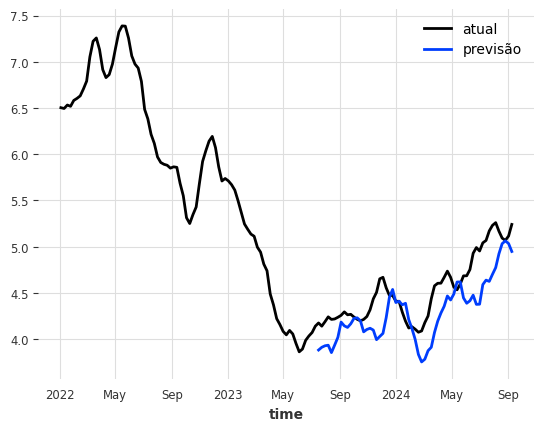
\includegraphics[width=\textwidth]{figuras/imp_brasil_plot.png} % Substitua pelo caminho da sua imagem
		\caption{Treinado com Biodiesel Nacional \newline}
		\label{fig:imp_brasil_plot}
	\end{subfigure}
	\hfill
	\begin{subfigure}[b]{0.45\textwidth}
		\centering
		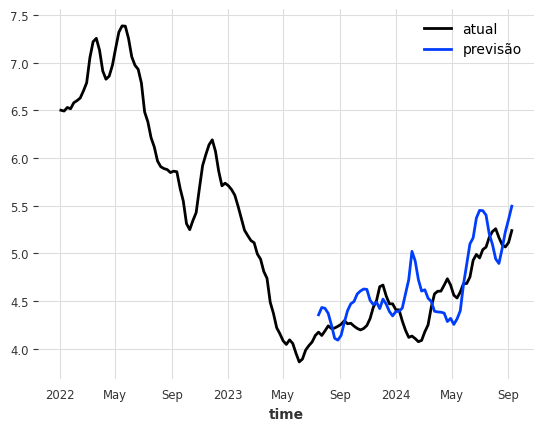
\includegraphics[width=\textwidth]{figuras/imp_brasil_oil_plot.png} % Substitua pelo caminho da sua imagem
		\caption{Treinado com Biodiesel Nacional e Óleo de Soja}
		\label{fig:imp_brasil_oil_plot}
	\end{subfigure}

	\vskip\baselineskip % Espaçamento vertical entre as linhas de imagens

	\begin{subfigure}[b]{0.45\textwidth}
		\centering
		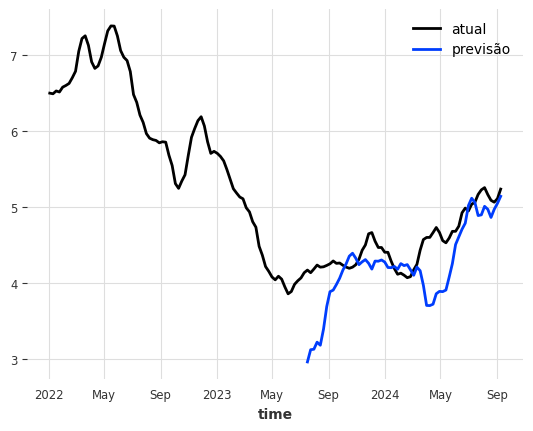
\includegraphics[width=\textwidth]{figuras/imp_brasil_detrend_plot.png} % Substitua pelo caminho da sua imagem
		\caption{Treinado com Biodiesel Nacional sem tendência}
		\label{fig:imp_brasil_detrend_plot}
	\end{subfigure}
	\hfill
	\begin{subfigure}[b]{0.45\textwidth}
		\centering
		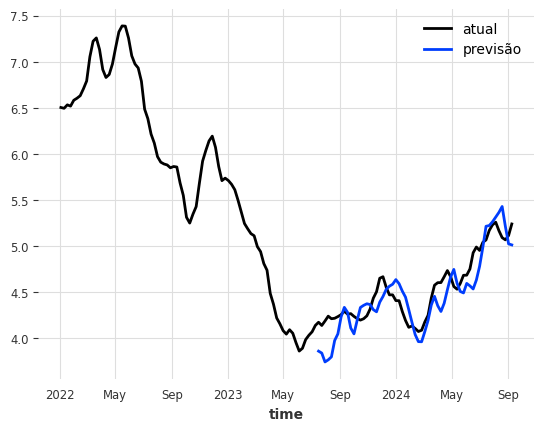
\includegraphics[width=\textwidth]{figuras/imp_brasil_oil_detrend_plot.png} % Substitua pelo caminho da sua imagem
		\caption{Treinado com Biodiesel Nacional e Óleo de Soja sem tendência}
		\label{fig:imp_brasil_oil_detrend_plot}
	\end{subfigure}

	\caption{Resultados do modelo \acs{IMP} no conjunto de teste}
	\label{fig:imp_results}
\end{figure}
\begin{figure}[htbp]
	\centering
	\begin{subfigure}[b]{0.40\textwidth}
		\centering
		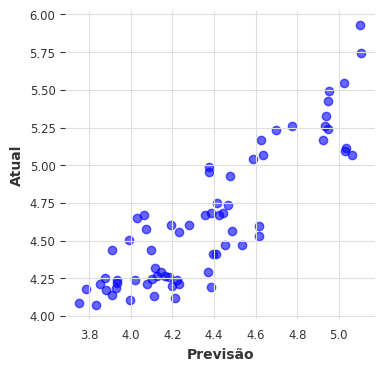
\includegraphics[width=\textwidth]{figuras/imp_brasil_scatter.png} % Substitua pelo caminho da sua imagem
		\caption{Treinado com Biodiesel Nacional \newline}
		\label{fig:imp_brasil_scatter}
	\end{subfigure}
	\hfill
	\begin{subfigure}[b]{0.40\textwidth}
		\centering
		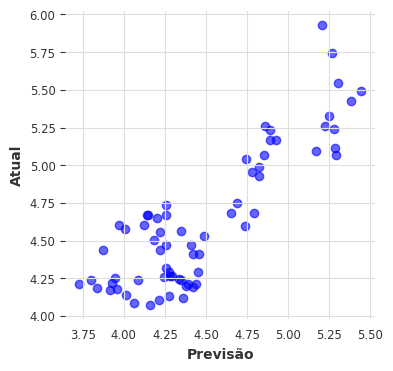
\includegraphics[width=\textwidth]{figuras/imp_brasil_oil_scatter.png} % Substitua pelo caminho da sua imagem
		\caption{Treinado com Biodiesel Nacional e Óleo de Soja}
		\label{fig:imp_brasil_oil_scatter}
	\end{subfigure}

	\vskip\baselineskip % Espaçamento vertical entre as linhas de imagens

	\begin{subfigure}[b]{0.40\textwidth}
		\centering
		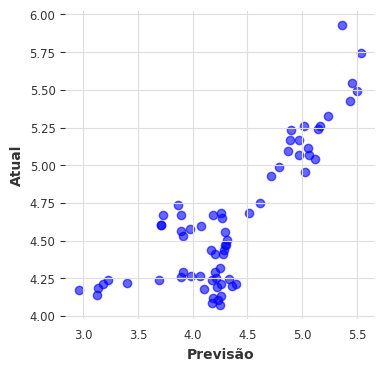
\includegraphics[width=\textwidth]{figuras/imp_brasil_detrend_scatter.png} % Substitua pelo caminho da sua imagem
		\caption{Treinado com Biodiesel Nacional sem tendência}
		\label{fig:imp_brasil_detrend_scatter}
	\end{subfigure}
	\hfill
	\begin{subfigure}[b]{0.40\textwidth}
		\centering
		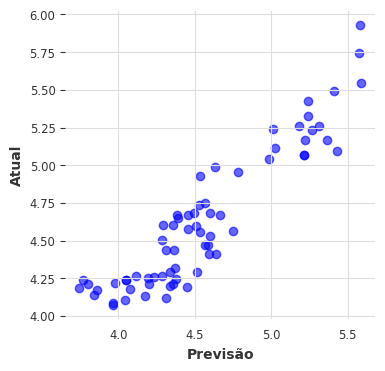
\includegraphics[width=\textwidth]{figuras/imp_brasil_oil_detrend_scatter.png} % Substitua pelo caminho da sua imagem
		\caption{Treinado com Biodiesel Nacional e Óleo de Soja sem tendência}
		\label{fig:imp_brasil_oil_detrend_scatter}
	\end{subfigure}

	\caption{Gráficos de dispersão dos valores atuais versus valores previstos pelo modelo \acs{IMP} no conjunto de teste}
	\label{fig:imp_scatter}
\end{figure}
\begin{figure}[htbp]
	\centering
	\begin{subfigure}[b]{0.40\textwidth}
		\centering
		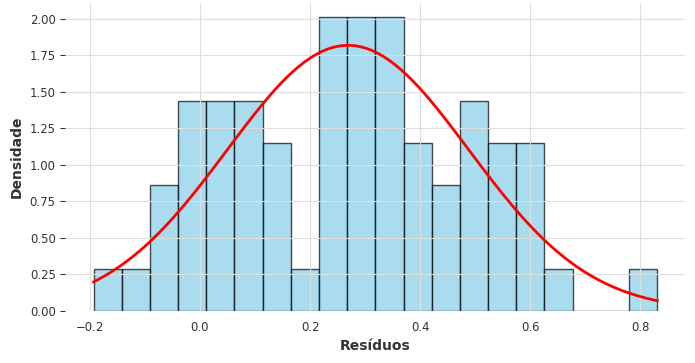
\includegraphics[width=\textwidth]{figuras/imp_brasil_residuals_histogram.png} % Substitua pelo caminho da sua imagem
		\caption{Treinado com Biodiesel Nacional \newline}
		\label{fig:imp_brasil_residuals_histogram}
	\end{subfigure}
	\hfill
	\begin{subfigure}[b]{0.40\textwidth}
		\centering
		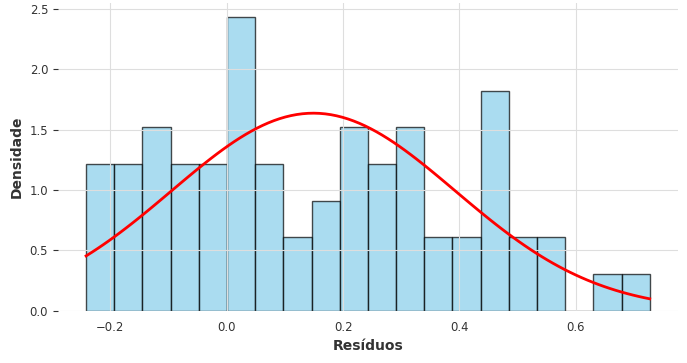
\includegraphics[width=\textwidth]{figuras/imp_brasil_oil_residuals_histogram.png} % Substitua pelo caminho da sua imagem
		\caption{Treinado com Biodiesel Nacional e Óleo de Soja}
		\label{fig:imp_brasil_oil_residuals_histogram}
	\end{subfigure}

	\vskip\baselineskip % Espaçamento vertical entre as linhas de imagens

	\begin{subfigure}[b]{0.40\textwidth}
		\centering
		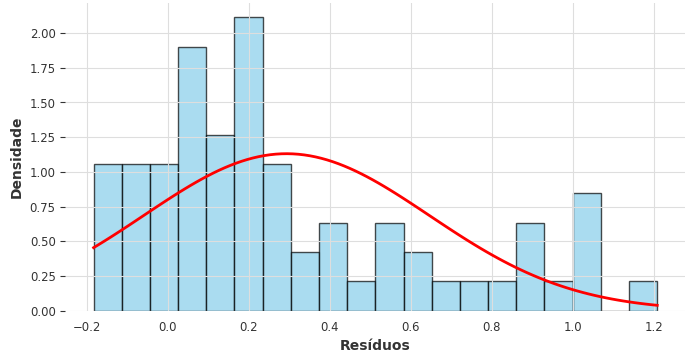
\includegraphics[width=\textwidth]{figuras/imp_brasil_detrend_residuals_histogram.png} % Substitua pelo caminho da sua imagem
		\caption{Treinado com Biodiesel Nacional sem tendência}
		\label{fig:imp_brasil_detrend_residuals_histogram}
	\end{subfigure}
	\hfill
	\begin{subfigure}[b]{0.40\textwidth}
		\centering
		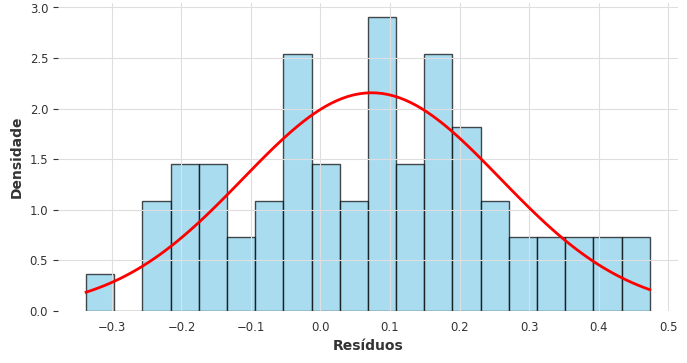
\includegraphics[width=\textwidth]{figuras/imp_brasil_oil_detrend_residuals_histogram.png} % Substitua pelo caminho da sua imagem
		\caption{Treinado com Biodiesel Nacional e Óleo de Soja sem tendência}
		\label{fig:imp_brasil_oil_detrend_residuals_histogram}
	\end{subfigure}

	\caption{Histograma dos erros do modelo \acs{IMP} no conjunto de teste}
	\label{fig:imp_residuals_histogram}
\end{figure}

\subsection{\acs{IDLN}}
\paragraph{} Conforme mostrado na Figura \ref{fig:idln_results}, os modelos (a) e (c) apresentaram bons resultados no conjunto de teste, embora tenham demonstrado inconsistência no conjunto de desenvolvimento, como evidenciado na Tabela \ref{tab:resultados_teste}. Essa discrepância pode indicar que, apesar de seu bom desempenho em condições controladas, esses modelos enfrentam dificuldades em generalizar adequadamente para dados não vistos durante o treinamento.
\paragraph{} Além disso, ao analisar os gráficos de dispersão apresentados na Figura \ref{fig:idln_scatter}, observou-se que os modelos (a) e (c) exibem uma dispersão reduzida, com uma correlação positiva clara entre os valores previstos e observados, embora o modelo (a) apresente uma correlação superior a 1. Em contraste, os modelos (b) e (d) apresentam uma dispersão maior, com uma correlação aparentemente não linear. O modelo (b), em particular, demonstrou uma alta dispersão.
\paragraph{} Por fim, ao examinar os histogramas apresentados na Figura \ref{fig:idln_residuals_histogram}, observou-se que o modelo (c) apresenta uma distribuição dos resíduos próxima a uma distribuição normal, enquanto os demais modelos exibem distribuições irregulares, com caudas pesadas e múltiplas modas.

\begin{figure}[htbp]
	\centering
	\begin{subfigure}[b]{0.45\textwidth}
		\centering
		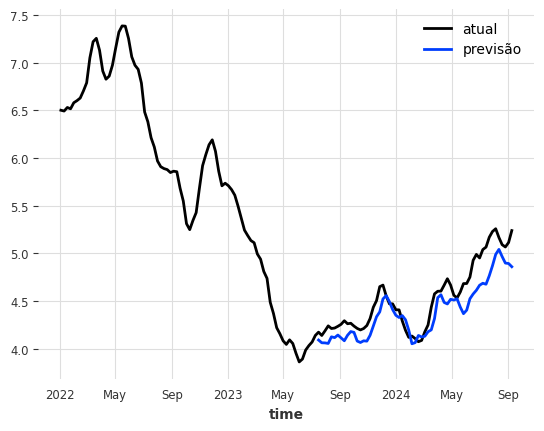
\includegraphics[width=\textwidth]{figuras/idln_brasil_plot.png} % Substitua pelo caminho da sua imagem
		\caption{Treinado com Biodiesel Nacional \newline}
		\label{fig:idln_brasil_plot}
	\end{subfigure}
	\hfill
	\begin{subfigure}[b]{0.45\textwidth}
		\centering
		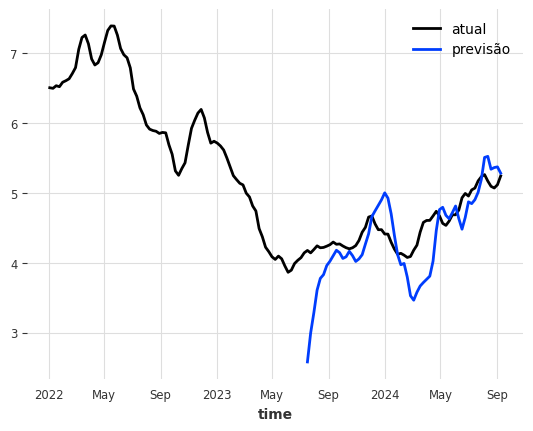
\includegraphics[width=\textwidth]{figuras/idln_brasil_oil_plot.png} % Substitua pelo caminho da sua imagem
		\caption{Treinado com Biodiesel Nacional e Óleo de Soja}
		\label{fig:idln_brasil_oil_plot}
	\end{subfigure}

	\vskip\baselineskip % Espaçamento vertical entre as linhas de imagens

	\begin{subfigure}[b]{0.45\textwidth}
		\centering
		\includegraphics[width=\textwidth]{figuras/idln_brasil_detrend_plot.png} % Substitua pelo caminho da sua imagem
		\caption{Treinado com Biodiesel Nacional sem tendência}
		\label{fig:idln_brasil_detrend_plot}
	\end{subfigure}
	\hfill
	\begin{subfigure}[b]{0.45\textwidth}
		\centering
		\includegraphics[width=\textwidth]{figuras/idln_brasil_oil_detrend_plot.png} % Substitua pelo caminho da sua imagem
		\caption{Treinado com Biodiesel Nacional e Óleo de Soja sem tendência}
		\label{fig:idln_brasil_oil_detrend_plot}
	\end{subfigure}
	\caption{Resultados do modelo \acs{IDLN} no conjunto de teste}

	\label{fig:idln_results}
\end{figure}
\begin{figure}[htbp]
	\centering
	\begin{subfigure}[b]{0.40\textwidth}
		\centering
		\includegraphics[width=\textwidth]{figuras/idln_brasil_scatter.png} % Substitua pelo caminho da sua imagem
		\caption{Treinado com Biodiesel Nacional \newline}
		\label{fig:idln_brasil_scatter}
	\end{subfigure}
	\hfill
	\begin{subfigure}[b]{0.40\textwidth}
		\centering
		\includegraphics[width=\textwidth]{figuras/idln_brasil_oil_scatter.png} % Substitua pelo caminho da sua imagem
		\caption{Treinado com Biodiesel Nacional e Óleo de Soja}
		\label{fig:idln_brasil_oil_scatter}
	\end{subfigure}

	\vskip\baselineskip % Espaçamento vertical entre as linhas de imagens

	\begin{subfigure}[b]{0.40\textwidth}
		\centering
		\includegraphics[width=\textwidth]{figuras/idln_brasil_detrend_scatter.png} % Substitua pelo caminho da sua imagem
		\caption{Treinado com Biodiesel Nacional sem tendência}
		\label{fig:idln_brasil_detrend_scatter}
	\end{subfigure}
	\hfill
	\begin{subfigure}[b]{0.40\textwidth}
		\centering
		\includegraphics[width=\textwidth]{figuras/idln_brasil_oil_detrend_scatter.png} % Substitua pelo caminho da sua imagem
		\caption{Treinado com Biodiesel Nacional e Óleo de Soja sem tendência}
		\label{fig:idln_brasil_oil_detrend_scatter}
	\end{subfigure}

	\caption{Gráficos de dispersão dos valores atuais versus valores previstos pelo modelo \acs{IDLN} no conjunto de teste}
	\label{fig:idln_scatter}
\end{figure}
\begin{figure}[htbp]
	\centering
	\begin{subfigure}[b]{0.40\textwidth}
		\centering
		\includegraphics[width=\textwidth]{figuras/idln_brasil_residuals_histogram.png} % Substitua pelo caminho da sua imagem
		\caption{Treinado com Biodiesel Nacional \newline}
		\label{fig:idln_brasil_residuals_histogram}
	\end{subfigure}
	\hfill
	\begin{subfigure}[b]{0.40\textwidth}
		\centering
		\includegraphics[width=\textwidth]{figuras/idln_brasil_oil_residuals_histogram.png} % Substitua pelo caminho da sua imagem
		\caption{Treinado com Biodiesel Nacional e Óleo de Soja}
		\label{fig:idln_brasil_oil_residuals_histogram}
	\end{subfigure}

	\vskip\baselineskip % Espaçamento vertical entre as linhas de imagens

	\begin{subfigure}[b]{0.40\textwidth}
		\centering
		\includegraphics[width=\textwidth]{figuras/idln_brasil_detrend_residuals_histogram.png} % Substitua pelo caminho da sua imagem
		\caption{Treinado com Biodiesel Nacional sem tendência}
		\label{fig:idln_brasil_detrend_residuals_histogram}
	\end{subfigure}
	\hfill
	\begin{subfigure}[b]{0.40\textwidth}
		\centering
		\includegraphics[width=\textwidth]{figuras/idln_brasil_oil_detrend_residuals_histogram.png} % Substitua pelo caminho da sua imagem
		\caption{Treinado com Biodiesel Nacional e Óleo de Soja sem tendência}
		\label{fig:idln_brasil_oil_detrend_residuals_histogram}
	\end{subfigure}

	\caption{Histograma dos erros do modelo \acs{IDLN} no conjunto de teste}
	\label{fig:idln_residuals_histogram}
\end{figure}

\subsection{\acs{N-Linear}}
\paragraph{} Conforme mostrado na Figura \ref{fig:nlinear_results}, os modelos (a) e (c) alcançaram um mapeamento próximo aos valores reais, destacando-se como os melhores no conjunto de teste. No entanto, de acordo com a Tabela \ref{tab:resultados_validacao}, esses resultados mostraram-se inconsistentes ao longo dos diferentes conjuntos de validação cruzada, sugerindo uma possível falta de robustez na generalização dos modelos para diferentes subconjuntos de dados.
\paragraph{} Além disso, a análise dos gráficos de dispersão apresentados na Figura \ref{fig:nlinear_scatter} revela que os modelos (a) e (c) apresentam baixa dispersão e uma clara correlação entre as previsões e os dados reais. Por outro lado, os modelos (b) e (d) exibem maior dispersão, embora ainda seja possível observar uma correlação positiva entre os valores previstos e observados.
\paragraph{} Por fim, ao examinar os histogramas apresentados na Figura \ref{fig:nlinear_residuals_histogram}, observou-se que o modelo (b) se aproxima de uma distribuição normal, enquanto os demais modelos apresentam um comportamento multimodal, com várias modas nas distribuições dos resíduos.

\begin{figure}[htbp]
	\centering
	\begin{subfigure}[b]{0.45\textwidth}
		\centering
		\includegraphics[width=\textwidth]{figuras/nlinear_brasil_plot.png} % Substitua pelo caminho da sua imagem
		\caption{Treinado com Biodiesel Nacional \newline}
		\label{fig:nlinear_brasil_plot}
	\end{subfigure}
	\hfill
	\begin{subfigure}[b]{0.45\textwidth}
		\centering
		\includegraphics[width=\textwidth]{figuras/nlinear_brasil_oil_plot.png} % Substitua pelo caminho da sua imagem
		\caption{Treinado com Biodiesel Nacional e Óleo de Soja}
		\label{fig:nlinear_brasil_oil_plot}
	\end{subfigure}

	\vskip\baselineskip % Espaçamento vertical entre as linhas de imagens

	\begin{subfigure}[b]{0.45\textwidth}
		\centering
		\includegraphics[width=\textwidth]{figuras/nlinear_brasil_detrend_plot.png} % Substitua pelo caminho da sua imagem
		\caption{Treinado com Biodiesel Nacional sem tendência}
		\label{fig:nlinear_brasil_detrend_plot}
	\end{subfigure}
	\hfill
	\begin{subfigure}[b]{0.45\textwidth}
		\centering
		\includegraphics[width=\textwidth]{figuras/nlinear_brasil_oil_detrend_plot.png} % Substitua pelo caminho da sua imagem
		\caption{Treinado com Biodiesel Nacional e Óleo de Soja sem tendência}
		\label{fig:nlinear_brasil_oil_detrend_plot}
	\end{subfigure}

	\caption{Resultados do modelo \acs{N-Linear} no conjunto de teste}
	\label{fig:nlinear_results}
\end{figure}
\begin{figure}[htbp]
	\centering
	\begin{subfigure}[b]{0.40\textwidth}
		\centering
		\includegraphics[width=\textwidth]{figuras/nlinear_brasil_scatter.png} % Substitua pelo caminho da sua imagem
		\caption{Treinado com Biodiesel Nacional \newline}
		\label{fig:nlinear_brasil_scatter}
	\end{subfigure}
	\hfill
	\begin{subfigure}[b]{0.40\textwidth}
		\centering
		\includegraphics[width=\textwidth]{figuras/nlinear_brasil_oil_scatter.png} % Substitua pelo caminho da sua imagem
		\caption{Treinado com Biodiesel Nacional e Óleo de Soja}
		\label{fig:nlinear_brasil_oil_scatter}
	\end{subfigure}

	\vskip\baselineskip % Espaçamento vertical entre as linhas de imagens

	\begin{subfigure}[b]{0.40\textwidth}
		\centering
		\includegraphics[width=\textwidth]{figuras/nlinear_brasil_detrend_scatter.png} % Substitua pelo caminho da sua imagem
		\caption{Treinado com Biodiesel Nacional sem tendência}
		\label{fig:nlinear_brasil_detrend_scatter}
	\end{subfigure}
	\hfill
	\begin{subfigure}[b]{0.40\textwidth}
		\centering
		\includegraphics[width=\textwidth]{figuras/nlinear_brasil_oil_detrend_scatter.png} % Substitua pelo caminho da sua imagem
		\caption{Treinado com Biodiesel Nacional e Óleo de Soja sem tendência}
		\label{fig:nlinear_brasil_oil_detrend_scatter}
	\end{subfigure}

	\caption{Gráficos de dispersão dos valores atuais versus valores previstos pelo modelo \acs{N-Linear} no conjunto de teste}
	\label{fig:nlinear_scatter}
\end{figure}
\begin{figure}[htbp]
	\centering
	\begin{subfigure}[b]{0.40\textwidth}
		\centering
		\includegraphics[width=\textwidth]{figuras/nlinear_brasil_residuals_histogram.png} % Substitua pelo caminho da sua imagem
		\caption{Treinado com Biodiesel Nacional \newline}
		\label{fig:nlinear_brasil_residuals_histogram}
	\end{subfigure}
	\hfill
	\begin{subfigure}[b]{0.40\textwidth}
		\centering
		\includegraphics[width=\textwidth]{figuras/nlinear_brasil_oil_residuals_histogram.png} % Substitua pelo caminho da sua imagem
		\caption{Treinado com Biodiesel Nacional e Óleo de Soja}
		\label{fig:nlinear_brasil_oil_residuals_histogram}
	\end{subfigure}

	\vskip\baselineskip % Espaçamento vertical entre as linhas de imagens

	\begin{subfigure}[b]{0.40\textwidth}
		\centering
		\includegraphics[width=\textwidth]{figuras/nlinear_brasil_detrend_residuals_histogram.png} % Substitua pelo caminho da sua imagem
		\caption{Treinado com Biodiesel Nacional sem tendência}
		\label{fig:nlinear_brasil_detrend_residuals_histogram}
	\end{subfigure}
	\hfill
	\begin{subfigure}[b]{0.40\textwidth}
		\centering
		\includegraphics[width=\textwidth]{figuras/nlinear_brasil_oil_detrend_residuals_histogram.png} % Substitua pelo caminho da sua imagem
		\caption{Treinado com Biodiesel Nacional e Óleo de Soja sem tendência}
		\label{fig:nlinear_brasil_oil_detrend_residuals_histogram}
	\end{subfigure}

	\caption{Histograma dos erros do modelo \acs{N-Linear} no conjunto de teste}
	\label{fig:nlinear_residuals_histogram}
\end{figure}

\subsection{\acs{NHiTS}}
\paragraph{} Conforme ilustrado na Figura \ref{fig:nhits_results}, o modelo (c) conseguiu mapear de forma próxima os valores reais, embora, segundo a Tabela \ref{tab:resultados_validacao}, esses resultados tenham se mostrado inconsistentes. Os modelos (b) e (c) demonstraram consistência ao longo da validação cruzada, conforme evidenciado na Tabela \ref{tab:resultados_validacao}, no entanto, ambos apresentaram desempenho inferior no conjunto de teste. Essa diferença entre os resultados de validação e teste sugere uma possível limitação na capacidade de generalização desses modelos quando expostos a dados não previamente vistos.
\paragraph{} Além disso, a análise dos gráficos de dispersão apresentados na Figura \ref{fig:nhits_scatter} revela uma clara correlação positiva em todos os modelos, embora com uma maior dispersão para valores menores.
\paragraph{} Ao examinar os histogramas da Figura \ref{fig:nhits_residuals_histogram}, observa-se que todos os modelos exibem mais de uma moda, indicando uma distribuição multimodal dos resíduos.

\begin{figure}[htbp]
	\centering
	\begin{subfigure}[b]{0.45\textwidth}
		\centering
		\includegraphics[width=\textwidth]{figuras/nhits_brasil_plot.png} % Substitua pelo caminho da sua imagem
		\caption{Treinado com Biodiesel Nacional \newline}
		\label{fig:nhits_brasil_plot}
	\end{subfigure}
	\hfill
	\begin{subfigure}[b]{0.45\textwidth}
		\centering
		\includegraphics[width=\textwidth]{figuras/nhits_brasil_oil_plot.png} % Substitua pelo caminho da sua imagem
		\caption{Treinado com Biodiesel Nacional e Óleo de Soja}
		\label{fig:nhits_brasil_oil_plot}
	\end{subfigure}

	\vskip\baselineskip % Espaçamento vertical entre as linhas de imagens

	\begin{subfigure}[b]{0.45\textwidth}
		\centering
		\includegraphics[width=\textwidth]{figuras/nhits_brasil_detrend_plot.png} % Substitua pelo caminho da sua imagem
		\caption{Treinado com Biodiesel Nacional sem tendência}
		\label{fig:nhits_brasil_detrend_plot}
	\end{subfigure}
	\hfill
	\begin{subfigure}[b]{0.45\textwidth}
		\centering
		\includegraphics[width=\textwidth]{figuras/nhits_brasil_oil_detrend_plot.png} % Substitua pelo caminho da sua imagem
		\caption{Treinado com Biodiesel Nacional e Óleo de Soja sem tendência}
		\label{fig:nhits_brasil_oil_detrend_plot}
	\end{subfigure}

	\caption{Resultados do modelo \acs{NHiTS} no conjunto de teste}
	\label{fig:nhits_results}
\end{figure}
\begin{figure}[htbp]
	\centering
	\begin{subfigure}[b]{0.40\textwidth}
		\centering
		\includegraphics[width=\textwidth]{figuras/nhits_brasil_scatter.png} % Substitua pelo caminho da sua imagem
		\caption{Treinado com Biodiesel Nacional \newline}
		\label{fig:nhits_brasil_scatter}
	\end{subfigure}
	\hfill
	\begin{subfigure}[b]{0.40\textwidth}
		\centering
		\includegraphics[width=\textwidth]{figuras/nhits_brasil_oil_scatter.png} % Substitua pelo caminho da sua imagem
		\caption{Treinado com Biodiesel Nacional e Óleo de Soja}
		\label{fig:nhits_brasil_oil_scatter}
	\end{subfigure}

	\vskip\baselineskip % Espaçamento vertical entre as linhas de imagens

	\begin{subfigure}[b]{0.40\textwidth}
		\centering
		\includegraphics[width=\textwidth]{figuras/nhits_brasil_detrend_scatter.png} % Substitua pelo caminho da sua imagem
		\caption{Treinado com Biodiesel Nacional sem tendência}
		\label{fig:nhits_brasil_detrend_scatter}
	\end{subfigure}
	\hfill
	\begin{subfigure}[b]{0.40\textwidth}
		\centering
		\includegraphics[width=\textwidth]{figuras/nhits_brasil_oil_detrend_scatter.png} % Substitua pelo caminho da sua imagem
		\caption{Treinado com Biodiesel Nacional e Óleo de Soja sem tendência}
		\label{fig:nhits_brasil_oil_detrend_scatter}
	\end{subfigure}

	\caption{Gráficos de dispersão dos valores atuais versus valores previstos pelo modelo \acs{NHiTS} no conjunto de teste}
	\label{fig:nhits_scatter}
\end{figure}
\begin{figure}[htbp]
	\centering
	\begin{subfigure}[b]{0.40\textwidth}
		\centering
		\includegraphics[width=\textwidth]{figuras/nhits_brasil_residuals_histogram.png} % Substitua pelo caminho da sua imagem
		\caption{Treinado com Biodiesel Nacional \newline}
		\label{fig:nhits_brasil_residuals_histogram}
	\end{subfigure}
	\hfill
	\begin{subfigure}[b]{0.40\textwidth}
		\centering
		\includegraphics[width=\textwidth]{figuras/nhits_brasil_oil_residuals_histogram.png} % Substitua pelo caminho da sua imagem
		\caption{Treinado com Biodiesel Nacional e Óleo de Soja}
		\label{fig:nhits_brasil_oil_residuals_histogram}
	\end{subfigure}

	\vskip\baselineskip % Espaçamento vertical entre as linhas de imagens

	\begin{subfigure}[b]{0.40\textwidth}
		\centering
		\includegraphics[width=\textwidth]{figuras/nhits_brasil_detrend_residuals_histogram.png} % Substitua pelo caminho da sua imagem
		\caption{Treinado com Biodiesel Nacional sem tendência}
		\label{fig:nhits_brasil_detrend_residuals_histogram}
	\end{subfigure}
	\hfill
	\begin{subfigure}[b]{0.40\textwidth}
		\centering
		\includegraphics[width=\textwidth]{figuras/nhits_brasil_oil_detrend_residuals_histogram.png} % Substitua pelo caminho da sua imagem
		\caption{Treinado com Biodiesel Nacional e Óleo de Soja sem tendência}
		\label{fig:nhits_brasil_oil_detrend_residuals_histogram}
	\end{subfigure}

	\caption{Histograma dos erros do modelo \acs{NHiTS} no conjunto de teste}
	\label{fig:nhits_residuals_histogram}
\end{figure}


\begin{table}[ht]
	\centering
	\caption{Resultados da Validação Cruzada usando Janela Deslizante}
	\label{tab:resultados_validacao}
	\begin{adjustbox}{angle=90, scale=0.63}
		\begin{tabular}{llcccccccccccc}
	\toprule
	\multicolumn{2}{c}{\textbf{Modelo}} & \multicolumn{6}{c}{\textbf{Biodiesel Nacional}} & \multicolumn{6}{c}{\textbf{Biodiesel Nacional + Óleo de Soja}}                                                                                                                                                                                                                                                                                                                                                                                                                                   \\
	\cmidrule(lr){3-8} \cmidrule(lr){9-14}
	                                    &                                                 & MAPE                                                           & SLE                                 & MSE                                 & RMSE                                & \(U_1\)                             & \(U_2\)                             & MAPE                                & SLE                                 & MSE                                 & RMSE                                & \(U_1\)                             & \(U_2\)                             \\
	\midrule
	\multirow{1}{*}{\ac{ARIMA}}
	                                    &                                                 & 15,79                                                          & 4,21                                & 0,87                                & 0,93                                & ---                                 & ---                                 & ---                                 & ---                                 & ---                                 & ---                                 & ---                                 & ---                                 \\
	\midrule
	\multirow{2}{*}{\ac{NARX}}
	                                    & Original                                        & \(5,72 \pm 0,56\)                                              & \(0,11 \pm 0,04\)                   & \(0,15 \pm 0,06\)                   & \(0,37 \pm 0,08\)                   & \(0,97 \pm 0,04\)                   & \(\mathbf{1,37} \pm \mathbf{0,49}\) & \(1,55 \pm 0,12\)                   & \(0,01 \pm 0,00\)                   & \(0,01 \pm 0,00\)                   & \(0,10 \pm 0,01\)                   & \(0,32 \pm 0,18\)                   & \(1,21 \pm 0,09\)                   \\
	                                    & Sem tendência                                   & \(9,68 \pm 5,26\)                                              & \(0,49 \pm 0,36\)                   & \(0,52 \pm 0,43\)                   & \(0,59 \pm 0,36\)                   & \(0,83 \pm 0,37\)                   & \(2,84 \pm 2,15\)                   & \(3,83 \pm 0,28\)                   & \(0,06 \pm 0,01\)                   & \(0,07 \pm 0,01\)                   & \(0,23 \pm 0,02\)                   & \(0,45 \pm 0,16\)                   & \(1,52 \pm 0,22\)                   \\
	\midrule
	\multirow{2}{*}{\ac{DA-RNN}}
	                                    & Original                                        & \(5,30 \pm 2,70\)                                              & \(0,11 \pm 0,09\)                   & \(0,16 \pm 0,14\)                   & \(0,34 \pm 0,20\)                   & \(0,70 \pm 0,01\)                   & \(3,91 \pm 0,97\)                   & \(1,93 \pm 0,07\)                   & \(0,01 \pm 0,00\)                   & \(0,01 \pm 0,00\)                   & \(0,12 \pm 0,02\)                   & \(0,36 \pm 0,17\)                   & \(1,80 \pm 0,04\)                   \\
	                                    & Sem tendência                                   & \(6,85 \pm 4,14\)                                              & \(0,25 \pm 0,22\)                   & \(0,30 \pm 0,28\)                   & \(0,45 \pm 0,31\)                   & \(0,74 \pm 0,37\)                   & \(2,73 \pm 0,51\)                   & \(1,82 \pm 0,33\)                   & \(0,01 \pm 0,00\)                   & \(0,01 \pm 0,01\)                   & \(0,11 \pm 0,03\)                   & \(\mathbf{0,18} \pm \mathbf{0,00}\) & \(0,97 \pm 0,14\)                   \\
	\midrule
	\multirow{2}{*}{\ac{MLP}}
	                                    & Original                                        & \(4,45 \pm 2,23\)                                              & \(0,10 \pm 0,08\)                   & \(0,12 \pm 0,11\)                   & \(0,30 \pm 0,18\)                   & \(0,80 \pm 0,10\)                   & \(1,74 \pm 0,37\)                   & \(1,27 \pm 0,02\)                   & \(\mathbf{0,01} \pm \mathbf{0,00}\) & \(\mathbf{0,01} \pm \mathbf{0,00}\) & \(\mathbf{0,08} \pm \mathbf{0,01}\) & \(0,27 \pm 0,13\)                   & \(0,93 \pm 0,05\)                   \\
	                                    & Sem tendência                                   & \(5,92 \pm 3,41\)                                              & \(0,15 \pm 0,13\)                   & \(0,19 \pm 0,17\)                   & \(0,37 \pm 0,23\)                   & \(0,60 \pm 0,28\)                   & \(1,60 \pm 0,68\)                   & \(1,55 \pm 0,11\)                   & \(0,01 \pm 0,00\)                   & \(0,01 \pm 0,00\)                   & \(0,10 \pm 0,01\)                   & \(0,19 \pm 0,05\)                   & \(0,48 \pm 0,22\)                   \\
	\midrule
	\multirow{2}{*}{\ac{IMP}}
	                                    & Original                                        & \(9,42 \pm 2,96\)                                              & \(0,27 \pm 0,14\)                   & \(0,38 \pm 0,26\)                   & \(0,57 \pm 0,23\)                   & \(0,87 \pm 0,15\)                   & \(5,75 \pm 1,24\)                   & \(4,15 \pm 0,20\)                   & \(0,06 \pm 0,01\)                   & \(0,07 \pm 0,02\)                   & \(0,25 \pm 0,05\)                   & \(0,67 \pm 0,27\)                   & \(2,24 \pm 0,55\)                   \\
	                                    & Sem tendência                                   & \(8,68 \pm 1,78\)                                              & \(0,39 \pm 0,12\)                   & \(0,38 \pm 0,22\)                   & \(0,59 \pm 0,18\)                   & \(1,03 \pm 0,14\)                   & \(1,84 \pm 0,19\)                   & \(6,20 \pm 0,02\)                   & \(0,14 \pm 0,01\)                   & \(0,17 \pm 0,04\)                   & \(0,41 \pm 0,05\)                   & \(0,54 \pm 0,01\)                   & \(1,80 \pm 0,77\)                   \\
	\midrule
	\multirow{2}{*}{\ac{IDLN}}
	                                    & Original                                        & \(4,99 \pm 2,47\)                                              & \(0,09 \pm 0,07\)                   & \(0,13 \pm 0,11\)                   & \(0,31 \pm 0,17\)                   & \(0,73 \pm 0,11\)                   & \(3,29 \pm 2,15\)                   & \(5,29 \pm 0,28\)                   & \(0,08 \pm 0,00\)                   & \(0,10 \pm 0,01\)                   & \(0,31 \pm 0,02\)                   & \(0,77 \pm 0,27\)                   & \(4,27 \pm 0,99\)                   \\
	                                    & Sem tendência                                   & \(4,85 \pm 2,31\)                                              & \(0,11 \pm 0,09\)                   & \(0,14 \pm 0,12\)                   & \(0,32 \pm 0,19\)                   & \(0,59 \pm 0,20\)                   & \(2,06 \pm 0,93\)                   & \(2,25 \pm 0,11\)                   & \(0,02 \pm 0,00\)                   & \(0,02 \pm 0,00\)                   & \(0,14 \pm 0,01\)                   & \(0,26 \pm 0,03\)                   & \(0,76 \pm 0,33\)                   \\
	\midrule
	\multirow{2}{*}{\ac{N-Linear}}
	                                    & Original                                        & \(\mathbf{3,09} \pm \mathbf{1,56}\)                            & \(\mathbf{0,05} \pm \mathbf{0,04}\) & \(\mathbf{0,06} \pm \mathbf{0,05}\) & \(\mathbf{0,21} \pm \mathbf{0,12}\) & \(0,47 \pm 0,03\)                   & \(2,28 \pm 1,07\)                   & \(1,41 \pm 0,13\)                   & \(0,01 \pm 0,00\)                   & \(0,01 \pm 0,00\)                   & \(0,09 \pm 0,02\)                   & \(0,28 \pm 0,14\)                   & \(1,04 \pm 0,06\)                   \\
	                                    & Sem tendência                                   & \(3,74 \pm 2,34\)                                              & \(0,10 \pm 0,09\)                   & \(0,12 \pm 0,11\)                   & \(0,28 \pm 0,20\)                   & \(\mathbf{0,36} \pm \mathbf{0,15}\) & \(1,85 \pm 1,38\)                   & \(1,33 \pm 0,10\)                   & \(0,01 \pm 0,00\)                   & \(0,01 \pm 0,00\)                   & \(0,09 \pm 0,02\)                   & \(0,18 \pm 0,02\)                   & \(\mathbf{0,31} \pm \mathbf{0,14}\) \\
	\midrule
	\multirow{2}{*}{\ac{NHiTS}}
	                                    & Original                                        & \(4,75 \pm 0,91\)                                              & \(0,09 \pm 0,05\)                   & \(0,11 \pm 0,07\)                   & \(0,31 \pm 0,12\)                   & \(0,95 \pm 0,05\)                   & \(2,05 \pm 1,02\)                   & \(\mathbf{1,27} \pm \mathbf{0,03}\) & \(0,01 \pm 0,00\)                   & \(0,01 \pm 0,00\)                   & \(0,09 \pm 0,01\)                   & \(0,28 \pm 0,15\)                   & \(1,08 \pm 0,03\)                   \\
	                                    & Sem tendência                                   & \(6,85 \pm 3,13\)                                              & \(0,22 \pm 0,16\)                   & \(0,25 \pm 0,21\)                   & \(0,44 \pm 0,24\)                   & \(0,82 \pm 0,24\)                   & \(1,75 \pm 0,70\)                   & \(1,38 \pm 0,08\)                   & \(0,01 \pm 0,00\)                   & \(0,01 \pm 0,00\)                   & \(0,09 \pm 0,01\)                   & \(0,18 \pm 0,04\)                   & \(0,50 \pm 0,10\)                   \\
	\bottomrule
\end{tabular}
	\end{adjustbox}
\end{table}
\begin{figure}[htbp]
	\centering
	% Primeira linha
	\begin{subfigure}[b]{0.3\textwidth}
		\centering
		\includegraphics[width=\textwidth]{figuras/mape_brasil_results.png}
		\caption{\ac{MAPE}}
		\label{fig:mape_brasil_results}
	\end{subfigure}
	\hfill
	\begin{subfigure}[b]{0.3\textwidth}
		\centering
		\includegraphics[width=\textwidth]{figuras/sle_brasil_results.png}
		\caption{\ac{SLE}}
		\label{fig:sle_brasil_results}
	\end{subfigure}
	\hfill
	\begin{subfigure}[b]{0.3\textwidth}
		\centering
		\includegraphics[width=\textwidth]{figuras/mse_brasil_results.png}
		\caption{\ac{MSE}}
		\label{fig:mse_brasil_results}
	\end{subfigure}

	\vskip\baselineskip % Espaçamento vertical entre as linhas

	% Segunda linha
	\begin{subfigure}[b]{0.3\textwidth}
		\centering
		\includegraphics[width=\textwidth]{figuras/rmse_brasil_results.png}
		\caption{\ac{RMSE}}
		\label{fig:rmse_brasil_results}
	\end{subfigure}
	\hfill
	\begin{subfigure}[b]{0.3\textwidth}
		\centering
		\includegraphics[width=\textwidth]{figuras/u1_brasil_results.png}
		\caption{\(U_1\)}
		\label{fig:u1_brasil_results}
	\end{subfigure}
	\hfill
	\begin{subfigure}[b]{0.3\textwidth}
		\centering
		\includegraphics[width=\textwidth]{figuras/u2_brasil_results.png}
		\caption{\(U_2\)}
		\label{fig:u2_brasil_results}
	\end{subfigure}
	\text{* sem tendência}
	\caption{Resultados da Validação Cruzada treinado com Biodiesel Nacional usando Janela Deslizante}
	\label{fig:brasil_results}
\end{figure}
\begin{figure}[htbp]
	\centering
	% Primeira linha
	\begin{subfigure}[b]{0.3\textwidth}
		\centering
		\includegraphics[width=\textwidth]{figuras/mape_brasil_oil_results.png}
		\caption{\ac{MAPE}}
		\label{fig:mape_brasil_oil_results}
	\end{subfigure}
	\hfill
	\begin{subfigure}[b]{0.3\textwidth}
		\centering
		\includegraphics[width=\textwidth]{figuras/sle_brasil_oil_results.png}
		\caption{\ac{SLE}}
		\label{fig:sle_brasil_oil_results}
	\end{subfigure}
	\hfill
	\begin{subfigure}[b]{0.3\textwidth}
		\centering
		\includegraphics[width=\textwidth]{figuras/mse_brasil_oil_results.png}
		\caption{\ac{MSE}}
		\label{fig:mse_brasil_oil_results}
	\end{subfigure}

	\vskip\baselineskip % Espaçamento vertical entre as linhas

	% Segunda linha
	\begin{subfigure}[b]{0.3\textwidth}
		\centering
		\includegraphics[width=\textwidth]{figuras/rmse_brasil_oil_results.png}
		\caption{\ac{RMSE}}
		\label{fig:rmse_brasil_oil_results}
	\end{subfigure}
	\hfill
	\begin{subfigure}[b]{0.3\textwidth}
		\centering
		\includegraphics[width=\textwidth]{figuras/u1_brasil_oil_results.png}
		\caption{\(U_1\)}
		\label{fig:u1_brasil_oil_results}
	\end{subfigure}
	\hfill
	\begin{subfigure}[b]{0.3\textwidth}
		\centering
		\includegraphics[width=\textwidth]{figuras/u2_brasil_oil_results.png}
		\caption{\(U_2\)}
		\label{fig:u2_brasil_oil_results}
	\end{subfigure}
	\text{* sem tendência}
	\caption{Resultados da Validação Cruzada treinado com Biodiesel Nacional e Óleo de Soja usando Janela Deslizante}
	\label{fig:brasil_oil_results}
\end{figure}
\begin{table}[ht]
	\centering
	\caption{Resultados do Conjunto de Teste usando Janela Deslizante}
	\label{tab:resultados_teste}
	\begin{adjustbox}{angle=90, scale=0.65}
		\begin{tabular}{llcccccccccccc}
	\toprule
	\multicolumn{2}{c}{\textbf{Modelo}} & \multicolumn{6}{c}{\textbf{Biodiesel Nacional}} & \multicolumn{6}{c}{\textbf{Biodiesel Nacional + Óleo de Soja}}                                                                                                                                                                                 \\
	\cmidrule(lr){3-8} \cmidrule(lr){9-14}
	                                    &                                                 & MAPE                                                           & SLE           & MSE           & RMSE          & \(U_1\)       & \(U_2\)       & MAPE          & SLE           & MSE           & RMSE          & \(U_1\)       & \(U_2\)       \\
	\midrule
	\multirow{2}{*}{\ac{NARX}}
	                                    & Original                                        & 6,25                                                           & 0,32          & 0,11          & 0,33          & 0,88          & 2,44          & 2,23          & 0,05          & 0,02          & 0,13          & \textbf{0,21} & 0,59          \\
	                                    & Sem tendência                                   & 4,97                                                           & 0,42          & 0,13          & 0,32          & 0,79          & 1,04          & 7,94          & 0,61          & 0,24          & 0,45          & 0,65          & 5,53          \\
	\midrule
	\multirow{2}{*}{\ac{DA-RNN}}
	                                    & Original                                        & 3,34                                                           & 0,11          & 0,04          & 0,20          & 0,30          & 1,90          & 3,61          & 0,13          & 0,05          & 0,22          & 0,35          & 2,75          \\
	                                    & Sem tendência                                   & 1,87                                                           & 0,03          & 0,01          & 0,10          & 0,27          & 0,64          & 5,13          & 0,31          & 0,09          & 0,30          & 0,81          & 1,48          \\
	\midrule
	\multirow{2}{*}{\ac{MLP}}
	                                    & Original                                        & 3,12                                                           & 0,09          & 0,03          & 0,18          & 0,32          & 2,00          & 6,91          & 0,40          & 0,14          & 0,37          & 0,69          & 2,10          \\
	                                    & Sem tendência                                   & 1,58                                                           & 0,02          & 0,01          & 0,09          & 0,24          & 0,21          & \textbf{1,62} & \textbf{0,02} & \textbf{0,01} & \textbf{0,09} & 0,23          & 0,52          \\
	\midrule
	\multirow{2}{*}{\ac{IMP}}
	                                    & Original                                        & 5,58                                                           & 0,31          & 0,10          & 0,31          & 0,57          & 2,31          & 5,69          & 0,29          & 0,10          & 0,31          & 0,43          & 9,15          \\
	                                    & Sem tendência                                   & 7,84                                                           & 0,90          & 0,23          & 0,48          & 1,08          & 1,15          & 3,73          & 0,13          & 0,04          & 0,20          & 0,55          & 1,70          \\
	\midrule
	\multirow{2}{*}{\ac{IDLN}}
	                                    & Original                                        & 3,42                                                           & 0,10          & 0,04          & 0,19          & 0,32          & 1,08          & 7,70          & 0,85          & 0,21          & 0,46          & 0,58          & 3,23          \\
	                                    & Sem tendência                                   & 1,66                                                           & 0,03          & 0,01          & 0,10          & 0,27          & 0,17          & 3,42          & 0,11          & 0,04          & 0,19          & 0,52          & \textbf{0,45} \\
	\midrule
	\multirow{2}{*}{\ac{N-Linear}}
	                                    & Original                                        & 1,72                                                           & 0,03          & 0,01          & 0,10          & \textbf{0,16} & 0,50          & 7,73          & 0,55          & 0,18          & 0,43          & 0,81          & 2,39          \\
	                                    & Sem tendência                                   & \textbf{1,47}                                                  & \textbf{0,02} & \textbf{0,01} & \textbf{0,09} & 0,22          & \textbf{0,10} & 4,34          & 0,21          & 0,06          & 0,25          & 0,64          & 0,70          \\
	\midrule
	\multirow{2}{*}{\ac{NHiTS}}
	                                    & Original                                        & 3,98                                                           & 0,15          & 0,05          & 0,23          & 0,41          & 2,06          & 5,23          & 0,25          & 0,09          & 0,30          & 0,54          & 1,96          \\
	                                    & Sem tendência                                   & 2,42                                                           & 0,06          & 0,02          & 0,14          & 0,39          & 0,19          & 4,42          & 0,23          & 0,07          & 0,26          & 0,77          & 0,50          \\
	\bottomrule
\end{tabular}
	\end{adjustbox}
\end{table}
\begin{figure}[htbp]
	\centering
	% Primeira linha
	\begin{subfigure}[b]{0.3\textwidth}
		\centering
		\includegraphics[width=\textwidth]{figuras/mape_brasil_results_test.png}
		\caption{\ac{MAPE}}
		\label{fig:mape_brasil_results_test}
	\end{subfigure}
	\hfill
	\begin{subfigure}[b]{0.3\textwidth}
		\centering
		\includegraphics[width=\textwidth]{figuras/sle_brasil_results_test.png}
		\caption{\ac{SLE}}
		\label{fig:sle_brasil_results_test}
	\end{subfigure}
	\hfill
	\begin{subfigure}[b]{0.3\textwidth}
		\centering
		\includegraphics[width=\textwidth]{figuras/mse_brasil_results_test.png}
		\caption{\ac{MSE}}
		\label{fig:mse_brasil_results_test}
	\end{subfigure}

	\vskip\baselineskip % Espaçamento vertical entre as linhas

	% Segunda linha
	\begin{subfigure}[b]{0.3\textwidth}
		\centering
		\includegraphics[width=\textwidth]{figuras/rmse_brasil_results_test.png}
		\caption{\ac{RMSE}}
		\label{fig:rmse_brasil_results_test}
	\end{subfigure}
	\hfill
	\begin{subfigure}[b]{0.3\textwidth}
		\centering
		\includegraphics[width=\textwidth]{figuras/u1_brasil_results_test.png}
		\caption{\(U_1\)}
		\label{fig:u1_brasil_results_test}
	\end{subfigure}
	\hfill
	\begin{subfigure}[b]{0.3\textwidth}
		\centering
		\includegraphics[width=\textwidth]{figuras/u2_brasil_results_test.png}
		\caption{\(U_2\)}
		\label{fig:u2_brasil_results_test}
	\end{subfigure}
	\text{* sem tendência}
	\caption{Resultados do Conjunto de Teste treinado com Biodiesel Nacional usando Janela Deslizante}
	\label{fig:brasil_results_test}
\end{figure}
\begin{figure}[htbp]
	\centering
	% Primeira linha
	\begin{subfigure}[b]{0.3\textwidth}
		\centering
		\includegraphics[width=\textwidth]{figuras/mape_brasil_oil_results_test.png}
		\caption{\ac{MAPE}}
		\label{fig:mape_brasil_oil_results_test}
	\end{subfigure}
	\hfill
	\begin{subfigure}[b]{0.3\textwidth}
		\centering
		\includegraphics[width=\textwidth]{figuras/sle_brasil_oil_results_test.png}
		\caption{\ac{SLE}}
		\label{fig:sle_brasil_oil_results_test}
	\end{subfigure}
	\hfill
	\begin{subfigure}[b]{0.3\textwidth}
		\centering
		\includegraphics[width=\textwidth]{figuras/mse_brasil_oil_results_test.png}
		\caption{\ac{MSE}}
		\label{fig:mse_brasil_oil_results_test}
	\end{subfigure}

	\vskip\baselineskip % Espaçamento vertical entre as linhas

	% Segunda linha
	\begin{subfigure}[b]{0.3\textwidth}
		\centering
		\includegraphics[width=\textwidth]{figuras/rmse_brasil_oil_results_test.png}
		\caption{\ac{RMSE}}
		\label{fig:rmse_brasil_oil_results_test}
	\end{subfigure}
	\hfill
	\begin{subfigure}[b]{0.3\textwidth}
		\centering
		\includegraphics[width=\textwidth]{figuras/u1_brasil_oil_results_test.png}
		\caption{\(U_1\)}
		\label{fig:u1_brasil_oil_results_test}
	\end{subfigure}
	\hfill
	\begin{subfigure}[b]{0.3\textwidth}
		\centering
		\includegraphics[width=\textwidth]{figuras/u2_brasil_oil_results_test.png}
		\caption{\(U_2\)}
		\label{fig:u2_brasil_oil_results_test}
	\end{subfigure}
	\text{* sem tendência}
	\caption{Resultados do Conjunto de Teste treinado com Biodiesel Nacional e Óleo de Soja usando Janela Deslizante}
	\label{fig:brasil_oil_results_test}
\end{figure}


\section{Janela de Takens}

\paragraph{} Os resultados obtidos pelo modelo utilizando a abordagem de janela de takens são apresentados nas Tabelas \ref{tab:resultados_validacao_takens} e \ref{tab:resultados_teste_takens}, que detalham as métricas de desempenho para cada cenário avaliado, tanto na validação cruzada quanto no conjunto de teste. Além disso, as Figuras \ref{fig:takens_brasil_results}, \ref{fig:takens_brasil_oil_results}, \ref{fig:takens_brasil_results_test} e \ref{fig:takens_brasil_oil_results_test} ilustram essa comparação de forma gráfica, representando os mesmos dados das tabelas em gráficos de pontos.
\paragraph{} As subseções a seguir discutem os resultados de cada modelo, abordando os gráficos de previsão e a distribuição dos resíduos. Serão apresentadas as previsões comparadas aos valores reais, além da análise da distribuição dos resíduos por meio de histogramas e gráficos de dispersão, com o objetivo de compreender o comportamento do modelo e avaliar sua adequação aos dados.

\subsection{\acs{NARX}}
\paragraph{} Conforme apresentado na Figura \ref{fig:narx_takens_results} mostra-se que o modelo (b) foi o único capaz de mapear os dados reais de forma satisfatória, apresentando baixos valores de erro no conjunto de teste e mantendo essa performance de forma consistente no conjunto de desenvolvimento. Os resultados obtidos indicam que o desvio padrão dos erros foi inferior a 10\% das respectivas medidas, como detalhado nas Tabelas \ref{tab:resultados_validacao_takens} e \ref{tab:resultados_teste_takens}. Os demais modelos apresentam resultados inconsistentes no conjunto de validação e altos valores de erro no conjunto de teste. 
\paragraph{} Além disso, ao avaliar os gráficos de dispersão apresentados na Figura \ref{fig:narx_takens_scatter}, observa-se que o modelo (b) apresenta uma correlação positiva clara entre os valores previstos e observados, com baixa dispersão. Em contrapartida, os modelos (a), (c) e (d) exibem maior dispersão, com uma correlação mais fraca entre os valores previstos e observados.
\paragraph{} Por fim, ao analisar os histogramas da Figura \ref{fig:narx_takens_residuals_histogram}, observa-se que os modelos (a), (c) e (d) apresentam distribuições dos resíduos que se aproximam de uma distribuição normal, enquanto o modelo (b) exibe uma distribuição com cauda longa, sugerindo a presença de valores extremos nos resíduos.


\begin{figure}[htbp]
	\centering
	\begin{subfigure}[b]{0.45\textwidth}
		\centering
		\includegraphics[width=\textwidth]{figuras/narx_takens_brasil_plot.png} % Substitua pelo caminho da sua imagem
		\caption{Treinado com Biodiesel Nacional \newline}
		\label{fig:narx_takens_brasil_plot}
	\end{subfigure}
	\hfill
	\begin{subfigure}[b]{0.45\textwidth}
		\centering
		\includegraphics[width=\textwidth]{figuras/narx_takens_brasil_oil_plot.png} % Substitua pelo caminho da sua imagem
		\caption{Treinado com Biodiesel Nacional e Óleo de Soja}
		\label{fig:narx_takens_brasil_oil_plot}
	\end{subfigure}

	\vskip\baselineskip % Espaçamento vertical entre as linhas de imagens

	\begin{subfigure}[b]{0.45\textwidth}
		\centering
		\includegraphics[width=\textwidth]{figuras/narx_takens_brasil_detrend_plot.png} % Substitua pelo caminho da sua imagem
		\caption{Treinado com Biodiesel Nacional sem tendência}
		\label{fig:narx_takens_brasil_detrend_plot}
	\end{subfigure}
	\hfill
	\begin{subfigure}[b]{0.45\textwidth}
		\centering
		\includegraphics[width=\textwidth]{figuras/narx_takens_brasil_oil_detrend_plot.png} % Substitua pelo caminho da sua imagem
		\caption{Treinado com Biodiesel Nacional e Óleo de Soja sem tendência}
		\label{fig:narx_takens_brasil_oil_detrend_plot}
	\end{subfigure}

	\caption{Resultados do modelo \acs{NARX} Takens no conjunto de teste}
	\label{fig:narx_takens_results}
\end{figure}
\begin{figure}[htbp]
	\centering
	\begin{subfigure}[b]{0.40\textwidth}
		\centering
		\includegraphics[width=\textwidth]{figuras/narx_takens_brasil_scatter.png} % Substitua pelo caminho da sua imagem
		\caption{Treinado com Biodiesel Nacional \newline}
		\label{fig:narx_takens_brasil_scatter}
	\end{subfigure}
	\hfill
	\begin{subfigure}[b]{0.40\textwidth}
		\centering
		\includegraphics[width=\textwidth]{figuras/narx_takens_brasil_oil_scatter.png} % Substitua pelo caminho da sua imagem
		\caption{Treinado com Biodiesel Nacional e Óleo de Soja}
		\label{fig:narx_takens_brasil_oil_scatter}
	\end{subfigure}

	\vskip\baselineskip % Espaçamento vertical entre as linhas de imagens

	\begin{subfigure}[b]{0.40\textwidth}
		\centering
		\includegraphics[width=\textwidth]{figuras/narx_takens_brasil_detrend_scatter.png} % Substitua pelo caminho da sua imagem
		\caption{Treinado com Biodiesel Nacional sem tendência}
		\label{fig:narx_takens_brasil_detrend_scatter}
	\end{subfigure}
	\hfill
	\begin{subfigure}[b]{0.40\textwidth}
		\centering
		\includegraphics[width=\textwidth]{figuras/narx_takens_brasil_oil_detrend_scatter.png} % Substitua pelo caminho da sua imagem
		\caption{Treinado com Biodiesel Nacional e Óleo de Soja sem tendência}
		\label{fig:narx_takens_brasil_oil_detrend_scatter}
	\end{subfigure}

	\caption{Gráficos de dispersão dos valores atuais versus valores previstos pelo modelo \acs{NARX} Takens no conjunto de teste}
	\label{fig:narx_takens_scatter}
\end{figure}
\begin{figure}[htbp]
	\centering
	\begin{subfigure}[b]{0.40\textwidth}
		\centering
		\includegraphics[width=\textwidth]{figuras/narx_takens_brasil_residuals_histogram.png} % Substitua pelo caminho da sua imagem
		\caption{Treinado com Biodiesel Nacional \newline}
		\label{fig:narx_takens_brasil_residuals_histogram}
	\end{subfigure}
	\hfill
	\begin{subfigure}[b]{0.40\textwidth}
		\centering
		\includegraphics[width=\textwidth]{figuras/narx_takens_brasil_oil_residuals_histogram.png} % Substitua pelo caminho da sua imagem
		\caption{Treinado com Biodiesel Nacional e Óleo de Soja}
		\label{fig:narx_takens_brasil_oil_residuals_histogram}
	\end{subfigure}

	\vskip\baselineskip % Espaçamento vertical entre as linhas de imagens

	\begin{subfigure}[b]{0.40\textwidth}
		\centering
		\includegraphics[width=\textwidth]{figuras/narx_takens_brasil_detrend_residuals_histogram.png} % Substitua pelo caminho da sua imagem
		\caption{Treinado com Biodiesel Nacional sem tendência}
		\label{fig:narx_takens_brasil_detrend_residuals_histogram}
	\end{subfigure}
	\hfill
	\begin{subfigure}[b]{0.40\textwidth}
		\centering
		\includegraphics[width=\textwidth]{figuras/narx_takens_brasil_oil_detrend_residuals_histogram.png} % Substitua pelo caminho da sua imagem
		\caption{Treinado com Biodiesel Nacional e Óleo de Soja sem tendência}
		\label{fig:narx_takens_brasil_oil_detrend_residuals_histogram}
	\end{subfigure}

	\caption{Histograma dos erros do modelo \acs{NARX} Takens no conjunto de teste}
	\label{fig:narx_takens_residuals_histogram}
\end{figure}

\subsection{\acs{DA-RNN}}
\paragraph{} Conforme mostrado na Tabela \ref{tab:resultados_teste_takens} e ilustrado na Figura \ref{fig:darnn_takens_results}, os modelos (b) e (c) obtiveram melhor resultado no conjunto de teste. Além disso, o modelo (b) também apresentou consistência na validação cruzada, como mostra a Tabela \ref{tab:resultados_validacao_takens}, indicando boa capacidade de generalização para diferentes conjuntos de dados.
\paragraph{} Além disso, ao analisar os gráficos de dispersão apresentados na Figura \ref{fig:darnn_takens_scatter}, observa-se que todos os modelos apresentam correlação positiva, embora os modelos (a) e (d) exibam maior dispersão, indicando uma maior variabilidade nos valores previstos em comparação aos demais.
\paragraph{} Por fim, ao avaliar os histogramas da Figura \ref{fig:darnn_takens_residuals_histogram}, observa-se que o modelo (c) apresenta uma distribuição dos resíduos que se aproxima de uma distribuição normal, sugerindo uma maior consistência nos erros de previsão. Em contraste, os modelos (a), (b) e (d) exibem distribuições com cauda longa, o que indica a presença de valores extremos nos resíduos.

\begin{figure}[htbp]
	\centering
	\begin{subfigure}[b]{0.45\textwidth}
		\centering
		\includegraphics[width=\textwidth]{figuras/darnn_takens_brasil_plot.png} % Substitua pelo caminho da sua imagem
		\caption{Treinado com Biodiesel Nacional \newline}
		\label{fig:darnn_takens_brasil_plot}
	\end{subfigure}
	\hfill
	\begin{subfigure}[b]{0.45\textwidth}
		\centering
		\includegraphics[width=\textwidth]{figuras/darnn_takens_brasil_oil_plot.png} % Substitua pelo caminho da sua imagem
		\caption{Treinado com Biodiesel Nacional e Óleo de Soja}
		\label{fig:darnn_takens_brasil_oil_plot}
	\end{subfigure}

	\vskip\baselineskip % Espaçamento vertical entre as linhas de imagens

	\begin{subfigure}[b]{0.45\textwidth}
		\centering
		\includegraphics[width=\textwidth]{figuras/darnn_takens_brasil_detrend_plot.png} % Substitua pelo caminho da sua imagem
		\caption{Treinado com Biodiesel Nacional sem tendência}
		\label{fig:darnn_takens_brasil_detrend_plot}
	\end{subfigure}
	\hfill
	\begin{subfigure}[b]{0.45\textwidth}
		\centering
		\includegraphics[width=\textwidth]{figuras/darnn_takens_brasil_oil_detrend_plot.png} % Substitua pelo caminho da sua imagem
		\caption{Treinado com Biodiesel Nacional e Óleo de Soja sem tendência}
		\label{fig:darnn_takens_brasil_oil_detrend_plot}
	\end{subfigure}

	\caption{Resultados do modelo \acs{DA-RNN} Takens no conjunto de teste}
	\label{fig:darnn_takens_results}
\end{figure}
\begin{figure}[htbp]
	\centering
	\begin{subfigure}[b]{0.40\textwidth}
		\centering
		\includegraphics[width=\textwidth]{figuras/darnn_takens_brasil_scatter.png} % Substitua pelo caminho da sua imagem
		\caption{Treinado com Biodiesel Nacional \newline}
		\label{fig:darnn_takens_brasil_scatter}
	\end{subfigure}
	\hfill
	\begin{subfigure}[b]{0.40\textwidth}
		\centering
		\includegraphics[width=\textwidth]{figuras/darnn_takens_brasil_oil_scatter.png} % Substitua pelo caminho da sua imagem
		\caption{Treinado com Biodiesel Nacional e Óleo de Soja}
		\label{fig:darnn_takens_brasil_oil_scatter}
	\end{subfigure}

	\vskip\baselineskip % Espaçamento vertical entre as linhas de imagens

	\begin{subfigure}[b]{0.40\textwidth}
		\centering
		\includegraphics[width=\textwidth]{figuras/darnn_takens_brasil_detrend_scatter.png} % Substitua pelo caminho da sua imagem
		\caption{Treinado com Biodiesel Nacional sem tendência}
		\label{fig:darnn_takens_brasil_detrend_scatter}
	\end{subfigure}
	\hfill
	\begin{subfigure}[b]{0.40\textwidth}
		\centering
		\includegraphics[width=\textwidth]{figuras/darnn_takens_brasil_oil_detrend_scatter.png} % Substitua pelo caminho da sua imagem
		\caption{Treinado com Biodiesel Nacional e Óleo de Soja sem tendência}
		\label{fig:darnn_takens_brasil_oil_detrend_scatter}
	\end{subfigure}

	\caption{Gráficos de dispersão dos valores atuais versus valores previstos pelo modelo \acs{DA-RNN} Takens no conjunto de teste}
	\label{fig:darnn_takens_scatter}
\end{figure}
\begin{figure}[htbp]
	\centering
	\begin{subfigure}[b]{0.40\textwidth}
		\centering
		\includegraphics[width=\textwidth]{figuras/darnn_takens_brasil_residuals_histogram.png} % Substitua pelo caminho da sua imagem
		\caption{Treinado com Biodiesel Nacional \newline}
		\label{fig:darnn_takens_brasil_residuals_histogram}
	\end{subfigure}
	\hfill
	\begin{subfigure}[b]{0.40\textwidth}
		\centering
		\includegraphics[width=\textwidth]{figuras/darnn_takens_brasil_oil_residuals_histogram.png} % Substitua pelo caminho da sua imagem
		\caption{Treinado com Biodiesel Nacional e Óleo de Soja}
		\label{fig:darnn_takens_brasil_oil_residuals_histogram}
	\end{subfigure}

	\vskip\baselineskip % Espaçamento vertical entre as linhas de imagens

	\begin{subfigure}[b]{0.40\textwidth}
		\centering
		\includegraphics[width=\textwidth]{figuras/darnn_takens_brasil_detrend_residuals_histogram.png} % Substitua pelo caminho da sua imagem
		\caption{Treinado com Biodiesel Nacional sem tendência}
		\label{fig:darnn_takens_brasil_detrend_residuals_histogram}
	\end{subfigure}
	\hfill
	\begin{subfigure}[b]{0.40\textwidth}
		\centering
		\includegraphics[width=\textwidth]{figuras/darnn_takens_brasil_oil_detrend_residuals_histogram.png} % Substitua pelo caminho da sua imagem
		\caption{Treinado com Biodiesel Nacional e Óleo de Soja sem tendência}
		\label{fig:darnn_takens_brasil_oil_detrend_residuals_histogram}
	\end{subfigure}

	\caption{Histograma dos erros do modelo \acs{DA-RNN} Takens no conjunto de teste}
	\label{fig:darnn_takens_residuals_histogram}
\end{figure}

\subsection{\acs{MLP}}
\paragraph{} O modelo \ac{MLP} apresentou bons resultados em todos os casos, com o modelo (b) possuindo o menor erro entre todos os outros da janela de takens, como mostra a Tabela \ref{tab:resultados_teste_takens} e na Figura \ref{fig:mlp_takens_results}. Além disso, possui um dos melhores erros de validação cruzada com a melhor consistência, conforme a Tabela \ref{tab:resultados_validacao_takens}. Esses resultados indicam uma capacidade robusta de generalização e precisão do modelo nesse contexto.
\paragraph{} Além disso, ao analisar os gráficos de dispersão apresentados na Figura \ref{fig:mlp_takens_scatter}, observa-se que todos os modelos apresentam correlação positiva, embora o modelo (a) apresente maior dispersão, indicando maior variabilidade nos valores previstos.
\paragraph{} Por fim, ao examinar os histogramas da Figura \ref{fig:mlp_takens_residuals_histogram}, observa-se que os modelos (b) e (c) apresentam distribuições dos resíduos que se aproximam de uma distribuição normal. Em contraste, o modelo (a) exibe uma distribuição irregular, enquanto o modelo (b) apresenta uma distribuição com múltiplos picos, sugerindo um comportamento multimodal nos resíduos.

\begin{figure}[htbp]
	\centering
	\begin{subfigure}[b]{0.45\textwidth}
		\centering
		\includegraphics[width=\textwidth]{figuras/mlp_takens_brasil_plot.png} % Substitua pelo caminho da sua imagem
		\caption{Treinado com Biodiesel Nacional \newline}
		\label{fig:mlp_takens_brasil_plot}
	\end{subfigure}
	\hfill
	\begin{subfigure}[b]{0.45\textwidth}
		\centering
		\includegraphics[width=\textwidth]{figuras/mlp_takens_brasil_oil_plot.png} % Substitua pelo caminho da sua imagem
		\caption{Treinado com Biodiesel Nacional e Óleo de Soja}
		\label{fig:mlp_takens_brasil_oil_plot}
	\end{subfigure}

	\vskip\baselineskip % Espaçamento vertical entre as linhas de imagens

	\begin{subfigure}[b]{0.45\textwidth}
		\centering
		\includegraphics[width=\textwidth]{figuras/mlp_takens_brasil_detrend_plot.png} % Substitua pelo caminho da sua imagem
		\caption{Treinado com Biodiesel Nacional sem tendência}
		\label{fig:mlp_takens_brasil_detrend_plot}
	\end{subfigure}
	\hfill
	\begin{subfigure}[b]{0.45\textwidth}
		\centering
		\includegraphics[width=\textwidth]{figuras/mlp_takens_brasil_oil_detrend_plot.png} % Substitua pelo caminho da sua imagem
		\caption{Treinado com Biodiesel Nacional e Óleo de Soja sem tendência}
		\label{fig:mlp_takens_brasil_oil_detrend_plot}
	\end{subfigure}

	\caption{Resultados do modelo \acs{MLP} Takens no conjunto de teste}
	\label{fig:mlp_takens_results}
\end{figure}
\begin{figure}[htbp]
	\centering
	\begin{subfigure}[b]{0.40\textwidth}
		\centering
		\includegraphics[width=\textwidth]{figuras/mlp_takens_brasil_scatter.png} % Substitua pelo caminho da sua imagem
		\caption{Treinado com Biodiesel Nacional \newline}
		\label{fig:mlp_takens_brasil_scatter}
	\end{subfigure}
	\hfill
	\begin{subfigure}[b]{0.40\textwidth}
		\centering
		\includegraphics[width=\textwidth]{figuras/mlp_takens_brasil_oil_scatter.png} % Substitua pelo caminho da sua imagem
		\caption{Treinado com Biodiesel Nacional e Óleo de Soja}
		\label{fig:mlp_takens_brasil_oil_scatter}
	\end{subfigure}

	\vskip\baselineskip % Espaçamento vertical entre as linhas de imagens

	\begin{subfigure}[b]{0.40\textwidth}
		\centering
		\includegraphics[width=\textwidth]{figuras/mlp_takens_brasil_detrend_scatter.png} % Substitua pelo caminho da sua imagem
		\caption{Treinado com Biodiesel Nacional sem tendência}
		\label{fig:mlp_takens_brasil_detrend_scatter}
	\end{subfigure}
	\hfill
	\begin{subfigure}[b]{0.40\textwidth}
		\centering
		\includegraphics[width=\textwidth]{figuras/mlp_takens_brasil_oil_detrend_scatter.png} % Substitua pelo caminho da sua imagem
		\caption{Treinado com Biodiesel Nacional e Óleo de Soja sem tendência}
		\label{fig:mlp_takens_brasil_oil_detrend_scatter}
	\end{subfigure}

	\caption{Gráficos de dispersão dos valores atuais versus valores previstos pelo modelo \acs{MLP} Takens no conjunto de teste}
	\label{fig:mlp_takens_scatter}
\end{figure}
\begin{figure}[htbp]
	\centering
	\begin{subfigure}[b]{0.40\textwidth}
		\centering
		\includegraphics[width=\textwidth]{figuras/mlp_takens_brasil_residuals_histogram.png} % Substitua pelo caminho da sua imagem
		\caption{Treinado com Biodiesel Nacional \newline}
		\label{fig:mlp_takens_brasil_residuals_histogram}
	\end{subfigure}
	\hfill
	\begin{subfigure}[b]{0.40\textwidth}
		\centering
		\includegraphics[width=\textwidth]{figuras/mlp_takens_brasil_oil_residuals_histogram.png} % Substitua pelo caminho da sua imagem
		\caption{Treinado com Biodiesel Nacional e Óleo de Soja}
		\label{fig:mlp_takens_brasil_oil_residuals_histogram}
	\end{subfigure}

	\vskip\baselineskip % Espaçamento vertical entre as linhas de imagens

	\begin{subfigure}[b]{0.40\textwidth}
		\centering
		\includegraphics[width=\textwidth]{figuras/mlp_takens_brasil_detrend_residuals_histogram.png} % Substitua pelo caminho da sua imagem
		\caption{Treinado com Biodiesel Nacional sem tendência}
		\label{fig:mlp_takens_brasil_detrend_residuals_histogram}
	\end{subfigure}
	\hfill
	\begin{subfigure}[b]{0.40\textwidth}
		\centering
		\includegraphics[width=\textwidth]{figuras/mlp_takens_brasil_oil_detrend_residuals_histogram.png} % Substitua pelo caminho da sua imagem
		\caption{Treinado com Biodiesel Nacional e Óleo de Soja sem tendência}
		\label{fig:mlp_takens_brasil_oil_detrend_residuals_histogram}
	\end{subfigure}

	\caption{Histograma dos erros do modelo \acs{MLP} Takens no conjunto de teste}
	\label{fig:mlp_takens_residuals_histogram}
\end{figure}

\subsection{\acs{IMP}}
\paragraph{} Os modelos \ac{IMP} apresentaram erros elevados, quando comparados a outros modelos. Além disso, o modelo apresenta resultados inconsistentes para cada conjunto de treinamento, como mostra a Tabela \ref{tab:resultados_validacao_takens} e ilustrado pela Figura \ref{fig:imp_takens_results}, indicando dificuldade da generalização dos dados de treinamento.
\paragraph{} Adicionalmente, ao analisar os gráficos de dispersão apresentados na Figura \ref{fig:imp_takens_scatter}, observa-se que, embora os modelos exibam correlação positiva, há uma grande dispersão, indicando maior variabilidade nos valores previstos. Os histogramas mostrados na Figura \ref{fig:imp_takens_residuals_histogram} revelam distribuições multimodais e com cauda longa, sugerindo a presença de valores extremos nos resíduos e uma estrutura complexa dos erros de previsão.

\begin{figure}[htbp]
	\centering
	\begin{subfigure}[b]{0.45\textwidth}
		\centering
		\includegraphics[width=\textwidth]{figuras/imp_takens_brasil_plot.png} % Substitua pelo caminho da sua imagem
		\caption{Treinado com Biodiesel Nacional \newline}
		\label{fig:imp_takens_brasil_plot}
	\end{subfigure}
	\hfill
	\begin{subfigure}[b]{0.45\textwidth}
		\centering
		\includegraphics[width=\textwidth]{figuras/imp_takens_brasil_oil_plot.png} % Substitua pelo caminho da sua imagem
		\caption{Treinado com Biodiesel Nacional e Óleo de Soja}
		\label{fig:imp_takens_brasil_oil_plot}
	\end{subfigure}

	\vskip\baselineskip % Espaçamento vertical entre as linhas de imagens

	\begin{subfigure}[b]{0.45\textwidth}
		\centering
		\includegraphics[width=\textwidth]{figuras/imp_takens_brasil_detrend_plot.png} % Substitua pelo caminho da sua imagem
		\caption{Treinado com Biodiesel Nacional sem tendência}
		\label{fig:imp_takens_brasil_detrend_plot}
	\end{subfigure}
	\hfill
	\begin{subfigure}[b]{0.45\textwidth}
		\centering
		\includegraphics[width=\textwidth]{figuras/imp_takens_brasil_oil_detrend_plot.png} % Substitua pelo caminho da sua imagem
		\caption{Treinado com Biodiesel Nacional e Óleo de Soja sem tendência}
		\label{fig:imp_takens_brasil_oil_detrend_plot}
	\end{subfigure}

	\caption{Resultados do modelo \acs{IMP} Takens no conjunto de teste}
	\label{fig:imp_takens_results}
\end{figure}
\begin{figure}[htbp]
	\centering
	\begin{subfigure}[b]{0.40\textwidth}
		\centering
		\includegraphics[width=\textwidth]{figuras/imp_takens_brasil_scatter.png} % Substitua pelo caminho da sua imagem
		\caption{Treinado com Biodiesel Nacional \newline}
		\label{fig:imp_takens_brasil_scatter}
	\end{subfigure}
	\hfill
	\begin{subfigure}[b]{0.40\textwidth}
		\centering
		\includegraphics[width=\textwidth]{figuras/imp_takens_brasil_oil_scatter.png} % Substitua pelo caminho da sua imagem
		\caption{Treinado com Biodiesel Nacional e Óleo de Soja}
		\label{fig:imp_takens_brasil_oil_scatter}
	\end{subfigure}

	\vskip\baselineskip % Espaçamento vertical entre as linhas de imagens

	\begin{subfigure}[b]{0.40\textwidth}
		\centering
		\includegraphics[width=\textwidth]{figuras/imp_takens_brasil_detrend_scatter.png} % Substitua pelo caminho da sua imagem
		\caption{Treinado com Biodiesel Nacional sem tendência}
		\label{fig:imp_takens_brasil_detrend_scatter}
	\end{subfigure}
	\hfill
	\begin{subfigure}[b]{0.40\textwidth}
		\centering
		\includegraphics[width=\textwidth]{figuras/imp_takens_brasil_oil_detrend_scatter.png} % Substitua pelo caminho da sua imagem
		\caption{Treinado com Biodiesel Nacional e Óleo de Soja sem tendência}
		\label{fig:imp_takens_brasil_oil_detrend_scatter}
	\end{subfigure}

	\caption{Gráficos de dispersão dos valores atuais versus valores previstos pelo modelo \acs{IMP} Takens no conjunto de teste}
	\label{fig:imp_takens_scatter}
\end{figure}
\begin{figure}[htbp]
	\centering
	\begin{subfigure}[b]{0.40\textwidth}
		\centering
		\includegraphics[width=\textwidth]{figuras/imp_takens_brasil_residuals_histogram.png} % Substitua pelo caminho da sua imagem
		\caption{Treinado com Biodiesel Nacional \newline}
		\label{fig:imp_takens_brasil_residuals_histogram}
	\end{subfigure}
	\hfill
	\begin{subfigure}[b]{0.40\textwidth}
		\centering
		\includegraphics[width=\textwidth]{figuras/imp_takens_brasil_oil_residuals_histogram.png} % Substitua pelo caminho da sua imagem
		\caption{Treinado com Biodiesel Nacional e Óleo de Soja}
		\label{fig:imp_takens_brasil_oil_residuals_histogram}
	\end{subfigure}

	\vskip\baselineskip % Espaçamento vertical entre as linhas de imagens

	\begin{subfigure}[b]{0.40\textwidth}
		\centering
		\includegraphics[width=\textwidth]{figuras/imp_takens_brasil_detrend_residuals_histogram.png} % Substitua pelo caminho da sua imagem
		\caption{Treinado com Biodiesel Nacional sem tendência}
		\label{fig:imp_takens_brasil_detrend_residuals_histogram}
	\end{subfigure}
	\hfill
	\begin{subfigure}[b]{0.40\textwidth}
		\centering
		\includegraphics[width=\textwidth]{figuras/imp_takens_brasil_oil_detrend_residuals_histogram.png} % Substitua pelo caminho da sua imagem
		\caption{Treinado com Biodiesel Nacional e Óleo de Soja sem tendência}
		\label{fig:imp_takens_brasil_oil_detrend_residuals_histogram}
	\end{subfigure}

	\caption{Histograma dos erros do modelo \acs{IMP} Takens no conjunto de teste}
	\label{fig:imp_takens_residuals_histogram}
\end{figure}

\subsection{\acs{IDLN}}
\paragraph{} O modelo (c) apresentou resultado satisfatório no conjunto de teste, como mostrado na Figura \ref{fig:idln_takens_results}. Apesar disso, o desempenho se mostra inconsistente, como visto na Tabela \ref{tab:resultados_validacao_takens}, com desvio padrão aproximadamente 50\% do valor da medida.
\paragraph{} Além disso, ao analisar os gráficos de dispersão apresentados na Figura \ref{fig:idln_takens_scatter}, observa-se que todos os modelos apresentam correlação positiva. No entanto, os modelos (a), (b) e (d) exibem maior dispersão, o que indica maior variabilidade nos valores previstos em comparação aos demais modelos.
\paragraph{} Por fim, ao examinar os histogramas apresentados na Figura \ref{fig:idln_takens_residuals_histogram}, observa-se que os modelos (a) e (c) apresentam distribuições dos resíduos que se aproximam de uma distribuição normal, sugerindo maior consistência nos erros de previsão. Em contraste, os modelos (b) e (d) exibem distribuições com cauda longa, indicando a presença de valores extremos nos resíduos.

\begin{figure}[htbp]
	\centering
	\begin{subfigure}[b]{0.45\textwidth}
		\centering
		\includegraphics[width=\textwidth]{figuras/idln_takens_brasil_plot.png} % Substitua pelo caminho da sua imagem
		\caption{Treinado com Biodiesel Nacional \newline}
		\label{fig:idln_takens_brasil_plot}
	\end{subfigure}
	\hfill
	\begin{subfigure}[b]{0.45\textwidth}
		\centering
		\includegraphics[width=\textwidth]{figuras/idln_takens_brasil_oil_plot.png} % Substitua pelo caminho da sua imagem
		\caption{Treinado com Biodiesel Nacional e Óleo de Soja}
		\label{fig:idln_takens_brasil_oil_plot}
	\end{subfigure}

	\vskip\baselineskip % Espaçamento vertical entre as linhas de imagens

	\begin{subfigure}[b]{0.45\textwidth}
		\centering
		\includegraphics[width=\textwidth]{figuras/idln_takens_brasil_detrend_plot.png} % Substitua pelo caminho da sua imagem
		\caption{Treinado com Biodiesel Nacional sem tendência}
		\label{fig:idln_takens_brasil_detrend_plot}
	\end{subfigure}
	\hfill
	\begin{subfigure}[b]{0.45\textwidth}
		\centering
		\includegraphics[width=\textwidth]{figuras/idln_takens_brasil_oil_detrend_plot.png} % Substitua pelo caminho da sua imagem
		\caption{Treinado com Biodiesel Nacional e Óleo de Soja sem tendência}
		\label{fig:idln_takens_brasil_oil_detrend_plot}
	\end{subfigure}

	\caption{Resultados do modelo \acs{IDLN} Takens no conjunto de teste}
	\label{fig:idln_takens_results}
\end{figure}
\begin{figure}[htbp]
	\centering
	\begin{subfigure}[b]{0.40\textwidth}
		\centering
		\includegraphics[width=\textwidth]{figuras/idln_takens_brasil_scatter.png} % Substitua pelo caminho da sua imagem
		\caption{Treinado com Biodiesel Nacional \newline}
		\label{fig:idln_takens_brasil_scatter}
	\end{subfigure}
	\hfill
	\begin{subfigure}[b]{0.40\textwidth}
		\centering
		\includegraphics[width=\textwidth]{figuras/idln_takens_brasil_oil_scatter.png} % Substitua pelo caminho da sua imagem
		\caption{Treinado com Biodiesel Nacional e Óleo de Soja}
		\label{fig:idln_takens_brasil_oil_scatter}
	\end{subfigure}

	\vskip\baselineskip % Espaçamento vertical entre as linhas de imagens

	\begin{subfigure}[b]{0.40\textwidth}
		\centering
		\includegraphics[width=\textwidth]{figuras/idln_takens_brasil_detrend_scatter.png} % Substitua pelo caminho da sua imagem
		\caption{Treinado com Biodiesel Nacional sem tendência}
		\label{fig:idln_takens_brasil_detrend_scatter}
	\end{subfigure}
	\hfill
	\begin{subfigure}[b]{0.40\textwidth}
		\centering
		\includegraphics[width=\textwidth]{figuras/idln_takens_brasil_oil_detrend_scatter.png} % Substitua pelo caminho da sua imagem
		\caption{Treinado com Biodiesel Nacional e Óleo de Soja sem tendência}
		\label{fig:idln_takens_brasil_oil_detrend_scatter}
	\end{subfigure}

	\caption{Gráficos de dispersão dos valores atuais versus valores previstos pelo modelo \acs{IDLN} Takens no conjunto de teste}
	\label{fig:idln_takens_scatter}
\end{figure}
\begin{figure}[htbp]
	\centering
	\begin{subfigure}[b]{0.40\textwidth}
		\centering
		\includegraphics[width=\textwidth]{figuras/idln_takens_brasil_residuals_histogram.png} % Substitua pelo caminho da sua imagem
		\caption{Treinado com Biodiesel Nacional \newline}
		\label{fig:idln_takens_brasil_residuals_histogram}
	\end{subfigure}
	\hfill
	\begin{subfigure}[b]{0.40\textwidth}
		\centering
		\includegraphics[width=\textwidth]{figuras/idln_takens_brasil_oil_residuals_histogram.png} % Substitua pelo caminho da sua imagem
		\caption{Treinado com Biodiesel Nacional e Óleo de Soja}
		\label{fig:idln_takens_brasil_oil_residuals_histogram}
	\end{subfigure}

	\vskip\baselineskip % Espaçamento vertical entre as linhas de imagens

	\begin{subfigure}[b]{0.40\textwidth}
		\centering
		\includegraphics[width=\textwidth]{figuras/idln_takens_brasil_detrend_residuals_histogram.png} % Substitua pelo caminho da sua imagem
		\caption{Treinado com Biodiesel Nacional sem tendência}
		\label{fig:idln_takens_brasil_detrend_residuals_histogram}
	\end{subfigure}
	\hfill
	\begin{subfigure}[b]{0.40\textwidth}
		\centering
		\includegraphics[width=\textwidth]{figuras/idln_takens_brasil_oil_detrend_residuals_histogram.png} % Substitua pelo caminho da sua imagem
		\caption{Treinado com Biodiesel Nacional e Óleo de Soja sem tendência}
		\label{fig:idln_takens_brasil_oil_detrend_residuals_histogram}
	\end{subfigure}

	\caption{Histograma dos erros do modelo \acs{IDLN} Takens no conjunto de teste}
	\label{fig:idln_takens_residuals_histogram}
\end{figure}

\subsection{\acs{N-Linear}}
\paragraph{} Os modelos \ac{N-Linear} apresentaram bons resultados no conjunto de teste, conforme mostrado na Tabela \ref{tab:resultados_validacao_takens} e ilustrado na Figura \ref{fig:nlinear_takens_results}. Apesar disso, apenas os modelos (b) e (c) apresentam resultados consistentes, mostrando que o modelo possui um número elevado de parâmetros e precisa de muitos dados para um treinamento efetivo.
\paragraph{} Além disso, ao analisar os gráficos de dispersão apresentados na Figura \ref{fig:nlinear_takens_scatter}, observa-se que todos os modelos apresentam correlação com os valores reais. No entanto, o modelo (d) exibe maior dispersão para valores menores que 4,75, indicando maior variabilidade nos valores previstos nesse intervalo.
\paragraph{} Por fim, ao examinar os histogramas apresentados na Figura \ref{fig:nlinear_takens_residuals_histogram}, observa-se distribuições assimétricas e multimodais, sugerindo a presença de múltiplos picos nas distribuições dos resíduos, o que pode indicar complexidades nos erros de previsão.


\begin{figure}[htbp]
	\centering
	\begin{subfigure}[b]{0.45\textwidth}
		\centering
		\includegraphics[width=\textwidth]{figuras/nlinear_takens_brasil_plot.png} % Substitua pelo caminho da sua imagem
		\caption{Treinado com Biodiesel Nacional \newline}
		\label{fig:nlinear_takens_brasil_plot}
	\end{subfigure}
	\hfill
	\begin{subfigure}[b]{0.45\textwidth}
		\centering
		\includegraphics[width=\textwidth]{figuras/nlinear_takens_brasil_oil_plot.png} % Substitua pelo caminho da sua imagem
		\caption{Treinado com Biodiesel Nacional e Óleo de Soja}
		\label{fig:nlinear_takens_brasil_oil_plot}
	\end{subfigure}

	\vskip\baselineskip % Espaçamento vertical entre as linhas de imagens

	\begin{subfigure}[b]{0.45\textwidth}
		\centering
		\includegraphics[width=\textwidth]{figuras/nlinear_takens_brasil_detrend_plot.png} % Substitua pelo caminho da sua imagem
		\caption{Treinado com Biodiesel Nacional sem tendência}
		\label{fig:nlinear_takens_brasil_detrend_plot}
	\end{subfigure}
	\hfill
	\begin{subfigure}[b]{0.45\textwidth}
		\centering
		\includegraphics[width=\textwidth]{figuras/nlinear_takens_brasil_oil_detrend_plot.png} % Substitua pelo caminho da sua imagem
		\caption{Treinado com Biodiesel Nacional e Óleo de Soja sem tendência}
		\label{fig:nlinear_takens_brasil_oil_detrend_plot}
	\end{subfigure}

	\caption{Resultados do modelo \acs{N-Linear} Takens no conjunto de teste}
	\label{fig:nlinear_takens_results}
\end{figure}
\begin{figure}[htbp]
	\centering
	\begin{subfigure}[b]{0.40\textwidth}
		\centering
		\includegraphics[width=\textwidth]{figuras/nlinear_takens_brasil_scatter.png} % Substitua pelo caminho da sua imagem
		\caption{Treinado com Biodiesel Nacional \newline}
		\label{fig:nlinear_takens_brasil_scatter}
	\end{subfigure}
	\hfill
	\begin{subfigure}[b]{0.40\textwidth}
		\centering
		\includegraphics[width=\textwidth]{figuras/nlinear_takens_brasil_oil_scatter.png} % Substitua pelo caminho da sua imagem
		\caption{Treinado com Biodiesel Nacional e Óleo de Soja}
		\label{fig:nlinear_takens_brasil_oil_scatter}
	\end{subfigure}

	\vskip\baselineskip % Espaçamento vertical entre as linhas de imagens

	\begin{subfigure}[b]{0.40\textwidth}
		\centering
		\includegraphics[width=\textwidth]{figuras/nlinear_takens_brasil_detrend_scatter.png} % Substitua pelo caminho da sua imagem
		\caption{Treinado com Biodiesel Nacional sem tendência}
		\label{fig:nlinear_takens_brasil_detrend_scatter}
	\end{subfigure}
	\hfill
	\begin{subfigure}[b]{0.40\textwidth}
		\centering
		\includegraphics[width=\textwidth]{figuras/nlinear_takens_brasil_oil_detrend_scatter.png} % Substitua pelo caminho da sua imagem
		\caption{Treinado com Biodiesel Nacional e Óleo de Soja sem tendência}
		\label{fig:nlinear_takens_brasil_oil_detrend_scatter}
	\end{subfigure}

	\caption{Gráficos de dispersão dos valores atuais versus valores previstos pelo modelo \acs{N-Linear} Takens no conjunto de teste}
	\label{fig:nlinear_takens_scatter}
\end{figure}
\begin{figure}[htbp]
	\centering
	\begin{subfigure}[b]{0.40\textwidth}
		\centering
		\includegraphics[width=\textwidth]{figuras/nlinear_takens_brasil_residuals_histogram.png} % Substitua pelo caminho da sua imagem
		\caption{Treinado com Biodiesel Nacional \newline}
		\label{fig:nlinear_takens_brasil_residuals_histogram}
	\end{subfigure}
	\hfill
	\begin{subfigure}[b]{0.40\textwidth}
		\centering
		\includegraphics[width=\textwidth]{figuras/nlinear_takens_brasil_oil_residuals_histogram.png} % Substitua pelo caminho da sua imagem
		\caption{Treinado com Biodiesel Nacional e Óleo de Soja}
		\label{fig:nlinear_takens_brasil_oil_residuals_histogram}
	\end{subfigure}

	\vskip\baselineskip % Espaçamento vertical entre as linhas de imagens

	\begin{subfigure}[b]{0.40\textwidth}
		\centering
		\includegraphics[width=\textwidth]{figuras/nlinear_takens_brasil_detrend_residuals_histogram.png} % Substitua pelo caminho da sua imagem
		\caption{Treinado com Biodiesel Nacional sem tendência}
		\label{fig:nlinear_takens_brasil_detrend_residuals_histogram}
	\end{subfigure}
	\hfill
	\begin{subfigure}[b]{0.40\textwidth}
		\centering
		\includegraphics[width=\textwidth]{figuras/nlinear_takens_brasil_oil_detrend_residuals_histogram.png} % Substitua pelo caminho da sua imagem
		\caption{Treinado com Biodiesel Nacional e Óleo de Soja sem tendência}
		\label{fig:nlinear_takens_brasil_oil_detrend_residuals_histogram}
	\end{subfigure}

	\caption{Histograma dos erros do modelo \acs{N-Linear} Takens no conjunto de teste}
	\label{fig:nlinear_takens_residuals_histogram}
\end{figure}

\subsection{\acs{NHiTS}}
\paragraph{} O modelo (b) obteve um bom resultado no conjunto de teste, como mostrado na Figura \ref{fig:nhits_takens_results}. Além disso, o modelo foi o de menor erro na validação cruzada de forma consistente, como mostrado na Tabela \ref{tab:resultados_validacao_takens}, demostrando a capacidade de generalização do modelo para conjuntos de tamanhos distintos.
\paragraph{} Além disso, ao analisar os gráficos de dispersão apresentados na Figura \ref{fig:nhits_takens_scatter}, observa-se que todos os modelos apresentam correlação positiva com os valores reais. No entanto, os modelos (a), (c) e (d) exibem maior dispersão, indicando maior variabilidade nos valores previstos em comparação ao modelo (b).
\paragraph{} Por fim, ao examinar os histogramas apresentados na Figura \ref{fig:nhits_takens_residuals_histogram}, observa-se distribuições multimodais e com cauda longa, sugerindo a presença de valores extremos nos resíduos e uma estrutura complexa dos erros de previsão.

\begin{figure}[htbp]
	\centering
	\begin{subfigure}[b]{0.45\textwidth}
		\centering
		\includegraphics[width=\textwidth]{figuras/nhits_takens_brasil_plot.png} % Substitua pelo caminho da sua imagem
		\caption{Treinado com Biodiesel Nacional \newline}
		\label{fig:nhits_takens_brasil_plot}
	\end{subfigure}
	\hfill
	\begin{subfigure}[b]{0.45\textwidth}
		\centering
		\includegraphics[width=\textwidth]{figuras/nhits_takens_brasil_oil_plot.png} % Substitua pelo caminho da sua imagem
		\caption{Treinado com Biodiesel Nacional e Óleo de Soja}
		\label{fig:nhits_takens_brasil_oil_plot}
	\end{subfigure}

	\vskip\baselineskip % Espaçamento vertical entre as linhas de imagens

	\begin{subfigure}[b]{0.45\textwidth}
		\centering
		\includegraphics[width=\textwidth]{figuras/nhits_takens_brasil_detrend_plot.png} % Substitua pelo caminho da sua imagem
		\caption{Treinado com Biodiesel Nacional sem tendência}
		\label{fig:nhits_takens_brasil_detrend_plot}
	\end{subfigure}
	\hfill
	\begin{subfigure}[b]{0.45\textwidth}
		\centering
		\includegraphics[width=\textwidth]{figuras/darnn_takens_brasil_oil_detrend_plot.png} % Substitua pelo caminho da sua imagem
		\caption{Treinado com Biodiesel Nacional e Óleo de Soja sem tendência}
		\label{fig:nhits_takens_brasil_oil_detrend_plot}
	\end{subfigure}

	\caption{Resultados do modelo \acs{NHiTS} Takens no conjunto de teste}
	\label{fig:nhits_takens_results}
\end{figure}
\begin{figure}[htbp]
	\centering
	\begin{subfigure}[b]{0.40\textwidth}
		\centering
		\includegraphics[width=\textwidth]{figuras/nhits_takens_brasil_scatter.png} % Substitua pelo caminho da sua imagem
		\caption{Treinado com Biodiesel Nacional \newline}
		\label{fig:nhits_takens_brasil_scatter}
	\end{subfigure}
	\hfill
	\begin{subfigure}[b]{0.40\textwidth}
		\centering
		\includegraphics[width=\textwidth]{figuras/nhits_takens_brasil_oil_scatter.png} % Substitua pelo caminho da sua imagem
		\caption{Treinado com Biodiesel Nacional e Óleo de Soja}
		\label{fig:nhits_takens_brasil_oil_scatter}
	\end{subfigure}

	\vskip\baselineskip % Espaçamento vertical entre as linhas de imagens

	\begin{subfigure}[b]{0.40\textwidth}
		\centering
		\includegraphics[width=\textwidth]{figuras/nhits_takens_brasil_detrend_scatter.png} % Substitua pelo caminho da sua imagem
		\caption{Treinado com Biodiesel Nacional sem tendência}
		\label{fig:nhits_takens_brasil_detrend_scatter}
	\end{subfigure}
	\hfill
	\begin{subfigure}[b]{0.40\textwidth}
		\centering
		\includegraphics[width=\textwidth]{figuras/nhits_takens_brasil_oil_detrend_scatter.png} % Substitua pelo caminho da sua imagem
		\caption{Treinado com Biodiesel Nacional e Óleo de Soja sem tendência}
		\label{fig:nhits_takens_brasil_oil_detrend_scatter}
	\end{subfigure}

	\caption{Gráficos de dispersão dos valores atuais versus valores previstos pelo modelo \acs{NHiTS} Takens no conjunto de teste}
	\label{fig:nhits_takens_scatter}
\end{figure}
\begin{figure}[htbp]
	\centering
	\begin{subfigure}[b]{0.40\textwidth}
		\centering
		\includegraphics[width=\textwidth]{figuras/nhits_takens_brasil_residuals_histogram.png} % Substitua pelo caminho da sua imagem
		\caption{Treinado com Biodiesel Nacional \newline}
		\label{fig:nhits_takens_brasil_residuals_histogram}
	\end{subfigure}
	\hfill
	\begin{subfigure}[b]{0.40\textwidth}
		\centering
		\includegraphics[width=\textwidth]{figuras/nhits_takens_brasil_oil_residuals_histogram.png} % Substitua pelo caminho da sua imagem
		\caption{Treinado com Biodiesel Nacional e Óleo de Soja}
		\label{fig:nhits_takens_brasil_oil_residuals_histogram}
	\end{subfigure}

	\vskip\baselineskip % Espaçamento vertical entre as linhas de imagens

	\begin{subfigure}[b]{0.40\textwidth}
		\centering
		\includegraphics[width=\textwidth]{figuras/nhits_takens_brasil_detrend_residuals_histogram.png} % Substitua pelo caminho da sua imagem
		\caption{Treinado com Biodiesel Nacional sem tendência}
		\label{fig:nhits_takens_brasil_detrend_residuals_histogram}
	\end{subfigure}
	\hfill
	\begin{subfigure}[b]{0.40\textwidth}
		\centering
		\includegraphics[width=\textwidth]{figuras/nhits_takens_brasil_oil_detrend_residuals_histogram.png} % Substitua pelo caminho da sua imagem
		\caption{Treinado com Biodiesel Nacional e Óleo de Soja sem tendência}
		\label{fig:nhits_takens_brasil_oil_detrend_residuals_histogram}
	\end{subfigure}

	\caption{Histograma dos erros do modelo \acs{NHiTS} Takens no conjunto de teste}
	\label{fig:nhits_takens_residuals_histogram}
\end{figure}

\begin{table}[ht]
	\centering
	\caption{Resultados da Validação Cruzada usando Janela de Takens}
	\label{tab:resultados_validacao_takens}
	\begin{adjustbox}{angle=90, scale=0.63}
		\begin{tabular}{llcccccccccccc}
	\toprule
	\multicolumn{2}{c}{\textbf{Modelo}} & \multicolumn{6}{c}{\textbf{Biodiesel Nacional}} & \multicolumn{6}{c}{\textbf{Biodiesel Nacional + Óleo de Soja}}                                                                                                                                                                                                                                                                                                                                                                                                                                   \\
	\cmidrule(lr){3-8} \cmidrule(lr){9-14}
	                                    &                                                 & MAPE                                                           & SLE                                 & MSE                                 & RMSE                                & \(U_1\)                             & \(U_2\)                             & MAPE                                & SLE                                 & MSE                                 & RMSE                                & \(U_1\)                             & \(U_2\)                             \\
	\midrule
	\multirow{1}{*}{\ac{ARIMA}}
	                                    &                                                 & 15,79                                                          & 4,21                                & 0,87                                & 0,93                                & ---                                 & ---                                 & ---                                 & ---                                 & ---                                 & ---                                 & ---                                 & ---                                 \\
	\midrule
	\multirow{2}{*}{\ac{NARX}}
	                                    & Original                                        & \(14,85 \pm 2,23\)                                             & \(3,88 \pm 0,89\)                   & \(0,80 \pm 0,39\)                   & \(0,82 \pm 0,24\)                   & \(1,05 \pm 0,07\)                   & \(2,49 \pm 0,70\)                   & \(1,51 \pm 0,12\)                   & \(0,01 \pm 0,00\)                   & \(0,01 \pm 0,00\)                   & \(0,10 \pm 0,01\)                   & \(0,31 \pm 0,16\)                   & \(0,79 \pm 0,09\)                   \\
	                                    & Sem tendência                                   & \(8,45 \pm 3,29\)                                              & \(1,83 \pm 1,15\)                   & \(0,35 \pm 0,26\)                   & \(0,50 \pm 0,23\)                   & \(0,82 \pm 0,21\)                   & \(\mathbf{1,43} \pm \mathbf{0,28}\) & \(6,65 \pm 0,13\)                   & \(0,73 \pm 0,04\)                   & \(0,19 \pm 0,05\)                   & \(0,40 \pm 0,05\)                   & \(0,57 \pm 0,08\)                   & \(6,92 \pm 5,53\)                   \\
	\midrule
	\multirow{2}{*}{\ac{DA-RNN}}
	                                    & Original                                        & \(\mathbf{3,58} \pm \mathbf{2,01}\)                            & \(\mathbf{0,05} \pm \mathbf{0,04}\) & \(\mathbf{0,07} \pm \mathbf{0,06}\) & \(\mathbf{0,22} \pm \mathbf{0,14}\) & \(0,60 \pm 0,09\)                   & \(1,87 \pm 0,48\)                   & \(2,05 \pm 0,15\)                   & \(0,02 \pm 0,00\)                   & \(0,02 \pm 0,01\)                   & \(0,13 \pm 0,02\)                   & \(0,40 \pm 0,17\)                   & \(1,95 \pm 0,56\)                   \\
	                                    & Sem tendência                                   & \(6,85 \pm 4,14\)                                              & \(0,25 \pm 0,22\)                   & \(0,30 \pm 0,28\)                   & \(0,45 \pm 0,31\)                   & \(0,74 \pm 0,37\)                   & \(2,73 \pm 0,51\)                   & \(1,82 \pm 0,33\)                   & \(0,01 \pm 0,00\)                   & \(0,01 \pm 0,01\)                   & \(0,11 \pm 0,03\)                   & \(\mathbf{0,18} \pm \mathbf{0,00}\) & \(0,97 \pm 0,14\)                   \\
	\midrule
	\multirow{2}{*}{\ac{MLP}}
	                                    & Original                                        & \(3,94 \pm 1,46\)                                              & \(0,08 \pm 0,06\)                   & \(0,10 \pm 0,08\)                   & \(0,27 \pm 0,14\)                   & \(0,76 \pm 0,01\)                   & \(1,93 \pm 0,28\)                   & \(1,33 \pm 0,00\)                   & \(\mathbf{0,01} \pm \mathbf{0,00}\) & \(\mathbf{0,01} \pm \mathbf{0,00}\) & \(\mathbf{0,09} \pm \mathbf{0,01}\) & \(0,28 \pm 0,14\)                   & \(1,07 \pm 0,04\)                   \\
	                                    & Sem tendência                                   & \(5,92 \pm 3,41\)                                              & \(0,15 \pm 0,13\)                   & \(0,19 \pm 0,17\)                   & \(0,37 \pm 0,23\)                   & \(0,60 \pm 0,28\)                   & \(1,60 \pm 0,68\)                   & \(1,55 \pm 0,11\)                   & \(0,01 \pm 0,00\)                   & \(0,01 \pm 0,00\)                   & \(0,10 \pm 0,01\)                   & \(0,19 \pm 0,05\)                   & \(0,48 \pm 0,22\)                   \\
	\midrule
	\multirow{2}{*}{\ac{IMP}}
	                                    & Original                                        & \(14,03 \pm 3,68\)                                             & \(0,55 \pm 0,29\)                   & \(0,87 \pm 0,61\)                   & \(0,86 \pm 0,35\)                   & \(0,96 \pm 0,11\)                   & \(10,72 \pm 1,01\)                  & \(3,21 \pm 0,81\)                   & \(0,03 \pm 0,01\)                   & \(0,04 \pm 0,03\)                   & \(0,20 \pm 0,07\)                   & \(0,55 \pm 0,20\)                   & \(1,09 \pm 0,19\)                   \\
	                                    & Sem tendência                                   & \(10,10 \pm 1,42\)                                             & \(0,47 \pm 0,21\)                   & \(0,50 \pm 0,27\)                   & \(0,68 \pm 0,20\)                   & \(1,00 \pm 0,27\)                   & \(2,19 \pm 1,70\)                   & \(6,20 \pm 0,02\)                   & \(0,14 \pm 0,01\)                   & \(0,17 \pm 0,04\)                   & \(0,41 \pm 0,05\)                   & \(0,54 \pm 0,01\)                   & \(1,80 \pm 0,77\)                   \\
	\midrule
	\multirow{2}{*}{\ac{IDLN}}
	                                    & Original                                        & \(10,37 \pm 7,41\)                                             & \(0,61 \pm 0,58\)                   & \(0,66 \pm 0,63\)                   & \(0,65 \pm 0,49\)                   & \(0,92 \pm 0,20\)                   & \(6,69 \pm 4,57\)                   & \(4,41 \pm 0,73\)                   & \(0,06 \pm 0,02\)                   & \(0,06 \pm 0,01\)                   & \(0,25 \pm 0,01\)                   & \(0,65 \pm 0,33\)                   & \(3,66 \pm 1,23\)                   \\
	                                    & Sem tendência                                   & \(4,85 \pm 2,31\)                                              & \(0,11 \pm 0,09\)                   & \(0,14 \pm 0,12\)                   & \(0,32 \pm 0,19\)                   & \(0,59 \pm 0,20\)                   & \(2,06 \pm 0,93\)                   & \(2,25 \pm 0,11\)                   & \(0,02 \pm 0,00\)                   & \(0,02 \pm 0,00\)                   & \(0,14 \pm 0,01\)                   & \(0,26 \pm 0,03\)                   & \(0,76 \pm 0,33\)                   \\
	\midrule
	\multirow{2}{*}{\ac{N-Linear}}
	                                    & Original                                        & \(5,80 \pm 4,31\)                                              & \(0,19 \pm 0,18\)                   & \(0,22 \pm 0,21\)                   & \(0,37 \pm 0,29\)                   & \(0,71 \pm 0,23\)                   & \(3,32 \pm 2,24\)                   & \(1,36 \pm 0,11\)                   & \(0,01 \pm 0,00\)                   & \(0,01 \pm 0,00\)                   & \(0,09 \pm 0,02\)                   & \(0,28 \pm 0,14\)                   & \(1,07 \pm 0,02\)                   \\
	                                    & Sem tendência                                   & \(3,74 \pm 2,34\)                                              & \(0,10 \pm 0,09\)                   & \(0,12 \pm 0,11\)                   & \(0,28 \pm 0,20\)                   & \(\mathbf{0,36} \pm \mathbf{0,15}\) & \(1,85 \pm 1,38\)                   & \(1,33 \pm 0,10\)                   & \(0,01 \pm 0,00\)                   & \(0,01 \pm 0,00\)                   & \(0,09 \pm 0,02\)                   & \(0,18 \pm 0,02\)                   & \(\mathbf{0,31} \pm \mathbf{0,14}\) \\
	\midrule
	\multirow{2}{*}{\ac{NHiTS}}
	                                    & Original                                        & \(4,60 \pm 0,56\)                                              & \(0,08 \pm 0,04\)                   & \(0,10 \pm 0,06\)                   & \(0,30 \pm 0,10\)                   & \(0,95 \pm 0,05\)                   & \(1,97 \pm 0,87\)                   & \(\mathbf{1,32} \pm \mathbf{0,01}\) & \(0,01 \pm 0,00\)                   & \(0,01 \pm 0,00\)                   & \(0,09 \pm 0,01\)                   & \(0,27 \pm 0,13\)                   & \(1,10 \pm 0,08\)                   \\
	                                    & Sem tendência                                   & \(6,85 \pm 3,13\)                                              & \(0,22 \pm 0,16\)                   & \(0,25 \pm 0,21\)                   & \(0,44 \pm 0,24\)                   & \(0,82 \pm 0,24\)                   & \(1,75 \pm 0,70\)                   & \(1,38 \pm 0,08\)                   & \(0,01 \pm 0,00\)                   & \(0,01 \pm 0,00\)                   & \(0,09 \pm 0,01\)                   & \(0,18 \pm 0,04\)                   & \(0,50 \pm 0,10\)                   \\
	\bottomrule
\end{tabular}
	\end{adjustbox}
\end{table}
\begin{figure}[htbp]
	\centering
	% Primeira linha
	\begin{subfigure}[b]{0.3\textwidth}
		\centering
		\includegraphics[width=\textwidth]{figuras/mape_takens_brasil_results.png}
		\caption{\ac{MAPE}}
		\label{fig:mape_takens_brasil_results}
	\end{subfigure}
	\hfill
	\begin{subfigure}[b]{0.3\textwidth}
		\centering
		\includegraphics[width=\textwidth]{figuras/sle_takens_brasil_results.png}
		\caption{\ac{SLE}}
		\label{fig:sle_takens_brasil_results}
	\end{subfigure}
	\hfill
	\begin{subfigure}[b]{0.3\textwidth}
		\centering
		\includegraphics[width=\textwidth]{figuras/mse_takens_brasil_results.png}
		\caption{\ac{MSE}}
		\label{fig:mse_takens_brasil_results}
	\end{subfigure}

	\vskip\baselineskip % Espaçamento vertical entre as linhas

	% Segunda linha
	\begin{subfigure}[b]{0.3\textwidth}
		\centering
		\includegraphics[width=\textwidth]{figuras/rmse_takens_brasil_results.png}
		\caption{\ac{RMSE}}
		\label{fig:rmse_takens_brasil_results}
	\end{subfigure}
	\hfill
	\begin{subfigure}[b]{0.3\textwidth}
		\centering
		\includegraphics[width=\textwidth]{figuras/u1_takens_brasil_results.png}
		\caption{\(U_1\)}
		\label{fig:u1_takens_brasil_results}
	\end{subfigure}
	\hfill
	\begin{subfigure}[b]{0.3\textwidth}
		\centering
		\includegraphics[width=\textwidth]{figuras/u2_takens_brasil_results.png}
		\caption{\(U_2\)}
		\label{fig:u2_takens_brasil_results}
	\end{subfigure}
	\text{* sem tendência}
	\caption{Resultados da Validação Cruzada treinado com Biodiesel Nacional usando Janela de Takens}
	\label{fig:takens_brasil_results}
\end{figure}
\begin{figure}[htbp]
	\centering
	% Primeira linha
	\begin{subfigure}[b]{0.3\textwidth}
		\centering
		\includegraphics[width=\textwidth]{figuras/mape_takens_brasil_oil_results.png}
		\caption{\ac{MAPE}}
		\label{fig:mape_takens_brasil_oil_results}
	\end{subfigure}
	\hfill
	\begin{subfigure}[b]{0.3\textwidth}
		\centering
		\includegraphics[width=\textwidth]{figuras/sle_takens_brasil_oil_results.png}
		\caption{\ac{SLE}}
		\label{fig:sle_takens_brasil_oil_results}
	\end{subfigure}
	\hfill
	\begin{subfigure}[b]{0.3\textwidth}
		\centering
		\includegraphics[width=\textwidth]{figuras/mse_takens_brasil_oil_results.png}
		\caption{\ac{MSE}}
		\label{fig:mse_takens_brasil_oil_results}
	\end{subfigure}

	\vskip\baselineskip % Espaçamento vertical entre as linhas

	% Segunda linha
	\begin{subfigure}[b]{0.3\textwidth}
		\centering
		\includegraphics[width=\textwidth]{figuras/rmse_takens_brasil_oil_results.png}
		\caption{\ac{RMSE}}
		\label{fig:rmse_takens_brasil_oil_results}
	\end{subfigure}
	\hfill
	\begin{subfigure}[b]{0.3\textwidth}
		\centering
		\includegraphics[width=\textwidth]{figuras/u1_takens_brasil_oil_results.png}
		\caption{\(U_1\)}
		\label{fig:u1_takens_brasil_oil_results}
	\end{subfigure}
	\hfill
	\begin{subfigure}[b]{0.3\textwidth}
		\centering
		\includegraphics[width=\textwidth]{figuras/u2_takens_brasil_oil_results.png}
		\caption{\(U_2\)}
		\label{fig:u2_takens_brasil_oil_results}
	\end{subfigure}
	\text{* sem tendência}
	\caption{Resultados da Validação Cruzada treinado com Biodiesel Nacional e Óleo de Soja usando Janela de Takens}
	\label{fig:takens_brasil_oil_results}
\end{figure}
\begin{table}[ht]
	\centering
	\caption{Resultados do Conjunto de Teste usando Janela de Takens}
	\label{tab:resultados_teste_takens}
	\begin{adjustbox}{angle=90, scale=0.65}
		\begin{tabular}{llcccccccccccc}
	\toprule
	\multicolumn{2}{c}{\textbf{Modelo}} & \multicolumn{6}{c}{\textbf{Biodiesel Nacional}} & \multicolumn{6}{c}{\textbf{Biodiesel Nacional + Óleo de Soja}}                                                                                                                                                                                 \\
	\cmidrule(lr){3-8} \cmidrule(lr){9-14}
	                                    &                                                 & MAPE                                                           & SLE           & MSE           & RMSE          & \(U_1\)       & \(U_2\)       & MAPE          & SLE           & MSE           & RMSE          & \(U_1\)       & \(U_2\)       \\
	\midrule
	\multirow{2}{*}{\ac{NARX}}
	                                    & Original                                        & 7,85                                                           & 7,37          & 0,24          & 0,43          & 0,95          & 1,77          & 1,28          & 0,02          & 0,01          & 0,08          & 0,11          & 0,84          \\
	                                    & Sem tendência                                   & 6,40                                                           & 4,01          & 0,19          & 0,39          & 0,83          & 2,11          & 6,71          & 2,60          & 0,22          & 0,42          & 0,60          & 4,08          \\
	\midrule
	\multirow{2}{*}{\ac{DA-RNN}}
	                                    & Original                                        & 3,68                                                           & 0,12          & 0,04          & 0,21          & 0,31          & 0,98          & 1,48          & 0,02          & 0,01          & 0,09          & 0,13          & 0,55          \\
	                                    & Sem tendência                                   & 1,87                                                           & 0,03          & 0,01          & 0,10          & 0,27          & 0,64          & 5,13          & 0,31          & 0,09          & 0,30          & 0,81          & 1,48          \\
	\midrule
	\multirow{2}{*}{\ac{MLP}}
	                                    & Original                                        & 3,10                                                           & 0,10          & 0,03          & 0,19          & 0,32          & 1,63          & \textbf{1,25} & \textbf{0,01} & \textbf{0,01} & \textbf{0,07} & \textbf{0,10} & 0,72          \\
	                                    & Sem tendência                                   & 1,58                                                           & 0,02          & 0,01          & 0,09          & 0,24          & 0,21          & 1,62          & 0,02          & 0,01          & 0,09          & 0,23          & 0,52          \\
	\midrule
	\multirow{2}{*}{\ac{IMP}}
	                                    & Original                                        & 6,64                                                           & 0,41          & 0,13          & 0,36          & 0,62          & 3,32          & 2,61          & 0,05          & 0,02          & 0,14          & 0,20          & 1,63          \\
	                                    & Sem tendência                                   & 4,99                                                           & 0,31          & 0,09          & 0,29          & 0,67          & 2,23          & 3,73          & 0,13          & 0,04          & 0,20          & 0,55          & 1,70          \\
	\midrule
	\multirow{2}{*}{\ac{IDLN}}
	                                    & Original                                        & 3,92                                                           & 0,15          & 0,05          & 0,23          & 0,41          & 2,22          & 2,28          & 0,05          & 0,02          & 0,13          & 0,22          & 2,76          \\
	                                    & Sem tendência                                   & 1,66                                                           & 0,03          & 0,01          & 0,10          & 0,27          & 0,17          & 3,42          & 0,11          & 0,04          & 0,19          & 0,52          & \textbf{0,45} \\
	\midrule
	\multirow{2}{*}{\ac{N-Linear}}
	                                    & Original                                        & 1,76                                                           & 0,03          & 0,01          & 0,10          & \textbf{0,16} & 0,56          & 1,35          & 0,02          & 0,01          & 0,08          & 0,11          & 0,53          \\
	                                    & Sem tendência                                   & \textbf{1,47}                                                  & \textbf{0,02} & \textbf{0,01} & \textbf{0,09} & 0,22          & \textbf{0,10} & 4,34          & 0,21          & 0,06          & 0,25          & 0,64          & 0,70          \\
	\midrule
	\multirow{2}{*}{\ac{NHiTS}}
	                                    & Original                                        & 4,00                                                           & 0,14          & 0,05          & 0,22          & 0,39          & 1,79          & 1,31          & 0,02          & 0,01          & 0,08          & 0,11          & 0,75          \\
	                                    & Sem tendência                                   & 2,42                                                           & 0,06          & 0,02          & 0,14          & 0,39          & 0,19          & 4,42          & 0,23          & 0,07          & 0,26          & 0,77          & 0,50          \\
	\bottomrule
\end{tabular}
	\end{adjustbox}
\end{table}
\begin{figure}[htbp]
	\centering
	% Primeira linha
	\begin{subfigure}[b]{0.3\textwidth}
		\centering
		\includegraphics[width=\textwidth]{figuras/mape_takens_brasil_results_test.png}
		\caption{\ac{MAPE}}
		\label{fig:mape_takens_brasil_results_test}
	\end{subfigure}
	\hfill
	\begin{subfigure}[b]{0.3\textwidth}
		\centering
		\includegraphics[width=\textwidth]{figuras/sle_takens_brasil_results_test.png}
		\caption{\ac{SLE}}
		\label{fig:sle_takens_brasil_results_test}
	\end{subfigure}
	\hfill
	\begin{subfigure}[b]{0.3\textwidth}
		\centering
		\includegraphics[width=\textwidth]{figuras/mse_takens_brasil_results_test.png}
		\caption{\ac{MSE}}
		\label{fig:mse_takens_brasil_results_test}
	\end{subfigure}

	\vskip\baselineskip % Espaçamento vertical entre as linhas

	% Segunda linha
	\begin{subfigure}[b]{0.3\textwidth}
		\centering
		\includegraphics[width=\textwidth]{figuras/rmse_takens_brasil_results_test.png}
		\caption{\ac{RMSE}}
		\label{fig:rmse_takens_brasil_results_test}
	\end{subfigure}
	\hfill
	\begin{subfigure}[b]{0.3\textwidth}
		\centering
		\includegraphics[width=\textwidth]{figuras/u1_takens_brasil_results_test.png}
		\caption{\(U_1\)}
		\label{fig:u1_takens_brasil_results_test}
	\end{subfigure}
	\hfill
	\begin{subfigure}[b]{0.3\textwidth}
		\centering
		\includegraphics[width=\textwidth]{figuras/u2_takens_brasil_results_test.png}
		\caption{\(U_2\)}
		\label{fig:u2_takens_brasil_results_test}
	\end{subfigure}
	\text{* sem tendência}
	\caption{Resultados do Conjunto de Teste treinado com Biodiesel Nacional usando Janela de Takens}
	\label{fig:takens_brasil_results_test}
\end{figure}
\begin{figure}[htbp]
	\centering
	% Primeira linha
	\begin{subfigure}[b]{0.3\textwidth}
		\centering
		\includegraphics[width=\textwidth]{figuras/mape_takens_brasil_oil_results_test.png}
		\caption{\ac{MAPE}}
		\label{fig:mape_takens_brasil_oil_results_test}
	\end{subfigure}
	\hfill
	\begin{subfigure}[b]{0.3\textwidth}
		\centering
		\includegraphics[width=\textwidth]{figuras/sle_takens_brasil_oil_results_test.png}
		\caption{\ac{SLE}}
		\label{fig:sle_takens_brasil_oil_results_test}
	\end{subfigure}
	\hfill
	\begin{subfigure}[b]{0.3\textwidth}
		\centering
		\includegraphics[width=\textwidth]{figuras/mse_takens_brasil_oil_results_test.png}
		\caption{\ac{MSE}}
		\label{fig:mse_takens_brasil_oil_results_test}
	\end{subfigure}

	\vskip\baselineskip % Espaçamento vertical entre as linhas

	% Segunda linha
	\begin{subfigure}[b]{0.3\textwidth}
		\centering
		\includegraphics[width=\textwidth]{figuras/rmse_takens_brasil_oil_results_test.png}
		\caption{\ac{RMSE}}
		\label{fig:rmse_takens_brasil_oil_results_test}
	\end{subfigure}
	\hfill
	\begin{subfigure}[b]{0.3\textwidth}
		\centering
		\includegraphics[width=\textwidth]{figuras/u1_takens_brasil_oil_results_test.png}
		\caption{\(U_1\)}
		\label{fig:u1_takens_brasil_oil_results_test}
	\end{subfigure}
	\hfill
	\begin{subfigure}[b]{0.3\textwidth}
		\centering
		\includegraphics[width=\textwidth]{figuras/u2_takens_brasil_oil_results_test.png}
		\caption{\(U_2\)}
		\label{fig:u2_takens_brasil_oil_results_test}
	\end{subfigure}
	\text{* sem tendência}
	\caption{Resultados do Conjunto de Teste treinado com Biodiesel Nacional e Óleo de Soja usando Janela de Takens}
	\label{fig:takens_brasil_oil_results_test}
\end{figure}
